\documentclass{iutbscthesis}
\usepackage{kantlipsum} % This package is used to generate place holder text. Remove it in the actual world.
\usepackage[linesnumbered,ruled,vlined]{algorithm2e}
\usepackage{adjustbox}
\usepackage{svg}

% The iutbscthesis uses biblatex for bibliography management.
% You can learn the basics of biblatex from:
% https://www.overleaf.com/learn/latex/Bibliography_management_with_biblatex
\addbibresource{citations.bib}

% The complete title of your thesis, mandatory
\title{A Data Driven Toggling Gain Complementary Filtering Approach for Orientation Estimation}

% Use the \addauthor command to keep adding authors with student ID
\addauthor{Samnun Azfar}{200041130}
\addauthor{Ramisa Zaman Audhi}{200041131}
\addauthor{Mir Md Inzamam}{200041240}

% Use the \supervisor command to define the supervisor with name, designation, and department
% There needs to be one and only one supervisor
\supervisor{Dr.\ Abu Raihan Md.\ Mostafa Kamal}{Professor}{Department of Computer Science and Engineering}

% Use the \addcosupervisor command to add a cosupervisor. There might be no cosupervisor at all
% In that case, just remove all of the \addcosupervisor commands.
\addcosupervisor{Mohammad Ishrak Abedin}{Lecturer}{Department of Computer Science and Engineering}


% Complete department name, mandatory
\department{Department of Computer Science and Engineering}

% Complete program name, mandatory
\program{BACHELOR OF SCIENCE IN COMPUTER SCIENCE AND ENGINEERING}

% Date (day, month name, and year) when the presentation took place, mandatory
\defensedate{29}{May}{2025}

\graphicspath{{figures/}}

\begin{document}

%-------------------------- FRONT MATTER --------------------------%

% Generate cover page of the report to be printed on the hard cover
\coverpage

% Switch to roman page numbering
\pagenumbering{roman}

% Generate the title leaf, mandatory
\titlepage

% Auto generate declaration of candidate based on previous info, mandatory
\declarationofcandidate

% Dedicate report to someone. You may add more sentences to it.
\dedicatedto{the cats of IUT}

\tableofcontents
\listoffigures
\listoftables

\clearpage

% Add abbreviations within this environment using the \abbr command
\begin{abbreviations}
    \abbr{MARG}{Magnetic Angular-Rate Gravity}
    \abbr{INS}{Inertial Navigation System}
    \abbr{CF}{Complemetary Filtering/Complemetary Fusion}
    \abbr{EKF}{Extended Kalman Filter}
    \abbr{ML}{Machine Learning}
    \abbr{BROAD}{Berlin Robust Orientation Assessment Dataset}
    \abbr{RANSAC}{RANdom SAmple Consensus}
    \abbr{IMU}{Inertial Measurement Unit}
    \abbr{MEMS}{Micro-Electro-Mechanical Systems}

\end{abbreviations}

% Any acknowledgement that you want to write goes in the following environment
% \begin{acknowledgement}

% I am profoundly grateful to my supervisor, Dr.\ Lou Natic, for his endless patience, insightful critiques, and for always knowing just when to say, ``Have you tried turning it off and on again?'' His expertise and encouragement were instrumental in the completion of this thesis.

% A special thanks to my co-supervisor, Dr.\ Sue Permann, who provided invaluable support and the occasional pep talk disguised as a lecture on time management. Her unwavering belief in my work kept me going, even when the only thing I believed in was the power of procrastination.

% Finally, to my parents, whose love and support have been a constant source of strength. Thank you for always being there, for pretending to understand my research when I rambled on, and for not asking too many questions about why I was still not employed after all these years.

% To all of you, I extend my heartfelt appreciation and a promise: next time, I will take fewer detours through the land of streaming services.
% \end{acknowledgement}

% Write your abstract here.
\begin{abstract}
One of the three goals of an Inertial Navigation System(INS) is to estimate the 3D orientation of
INS given accelerometer, magnetometer and angular rate gyroscope readings. Complementary fusion 
is one of the most robust, mathematically simple and fast algorithms for fusing the accelerometer,
magnetometer and angular rate gyroscope readings to estimate the 3D orientation. But complementary
fusion of sensor data suffers from linear accelerations and constant gain problems. This thesis aims 
to solve the aforementioned issues in a data driven approach. Our thesis proposes a data driven toggling
scheme for the gain parameter and also proposes a data driven noise removal approach through a tree based
machine learning model. The variable gain decides trust of fusion between the sensors and the 
denoising ensures extraneous linear accelerations and magnetic disturbances are eleminated. Furthermore, the 
proposed algorithm is tested on a real-world dataset, and also we look forward to construct a device
to further test our proposed algorithm on a real-world scenario.
\end{abstract}

%-------------------------- MAIN BODY --------------------------%
% Switch to arabic page numbering
\pagenumbering{arabic}

\chapter{Introduction}

\section{Inertial Navigation and MARG Sensors} \label{introINSMARG}
Inertial Navigation refers the process of determining the \textit{position}, \textit{velocity} and \textit{orientation} of an object to relative to its initial navigation parameters, without the assistance of any position fixing devices located externally \cite{el2020inertial}. Any system estimating position, orientation or velocity of an object using Inertial Sensing is referred to as the Inertial Navigation System(INS). 
\par
The INS uses a multitude of sensors to predict the position, orientation or the velocity. Two of these sensors are common to almost all of these systems, which are the Gravity Sensor(senses the direction of gravitational acceleration vector) and the Gyrosope(Angular Rate Sensor). Optionally some systems include the Magnetometer sensor(senses the direction of the Magnetic North)\cite{nawrat2012inertial}.Together they are referred to as the \textbf{MARG} sensors.
\par
The INS faces significant amount of challenges while solving its 3 problems - \textbf{position estimation},\textbf{veloicty estimation} and \textbf{orientation estimation}. Low cost MARG sensors are subject to electrical disturbances and noises \cite{guo2017novel}\cite{hu2014robust}.The angular-rate sensor is subject to random noises and drift( a phenomenon where low frequency noises integrate over time and skew the estimates)\cite{guo2017novel}. Accelerometers suffer from linear-accelerations, where the linear acceleration becomes harder to distinguish from the gravitational vector\cite{hu2014robust}.

\section{Orientation Estimation and MARG Sensors}
Orientation Estimation is one of the 3 problems that an INS has to solve. 
Orientation of a 3d object could be represented by Euler Angles, 
Rotation Matrices, or quaternions\cite{attitudeREpresntation}. An 
orientation estimation algorithm is fed with the MARG sensor readings 
and it estimates the orientation of an object in 3D space, representing 
it in Euler angles, quaternions or through a rotation matrix.
\par
Any orientation estimation algorithm has to overcome the shortcomings of MARG 
sensors mentioned in \ref{introINSMARG}. Some popular algorithms are the Madgwick 
filter\cite{madgwick2011estimation}, Mahony filter\cite{mahony2008nonlinear}, EKF 
filter\cite{EKF}, Complementary filter\cite{compfilter}. Each algorithm employs 
distinct methodologies to mitigate the effects of sensor disturbances and enhance 
orientation estimation accuracy.

Our focus in this thesis would be to work with orientation estimation through the utilization of
MARG sensor readings.

\section{Orientation Estimation through Complementary Fusion}\label{section:CF}

The complementary filter is one of the most basic form of fusion where the orientation estimates of the Angular Rate-Gyros are fused with the estimates generated from the accelerometer and if available the magnetometer.
The basic complementary filtering\cite{forbes2015fundamentals}\cite{euston2008complementary} is represented as:
\begin{equation}
    R = (1-\alpha)R_g + \alpha R_{am}
\end{equation}
Where $R$ is the rotation estimation, $R_g$ is the rotation estimation from the 
rate-gyros and $R_{am}$ is the rotation estimate from the accelerometer 
and the magnetometer.$R$ being the rotation estimate can be represented in multiple forms
such as Euler angles, quaternion or as a rotation matrix.
\par
\subsection{Key Strengths of CF}
\begin{itemize}
    \item Reduced Calculation and computation, simple mathematical model.
    \item Faster convergence compared to Madgwick and EKF Filters\cite{valenti2015keeping}.
\end{itemize}
\subsection{Weaknesses of CF}
\begin{itemize}
    \item The value of the gain $\alpha$ is constant.
    \item Cannot efficiently differentiate between linear acceleration and gravitational acceleration.
\end{itemize}


\section{Our Goal- Overcoming the negatives of CF: A data driven approach}
\par
As discussed in \autoref{section:CF}, complementary filters (CF) offer notable 
advantages over existing orientation estimation algorithms. 
The objective of this thesis is to address the limitations of CF by utilizing data-driven approaches. Specifically, our goals are to:

\begin{itemize}
    \item Develop an ML model to dynamically adjust the parameter $\alpha$ based on MARG sensor measurements, enabling differentiation between low and high linear acceleration scenarios.Such methods have been studied in previous researches in \cite{vertzberger2022adaptive}.
    \item Train a predictive model to estimate and compensate for noise in MARG sensor data. Similar approaches found as \cite{denoising} and \cite{noiseremoval2}.
\end{itemize}

Through these improvements, we aim to improve the performance of CF, mitigating its weaknesses and placing it as a robust and competitive algorithm for orientation estimation.


\section{Organization}

After this introduction , we elaborate on some of the related 
works 
that have been done on this field in \autoref{chapter:RelatedWorks}. 
Then we describe our proposed methodology in \autoref{chapter:proposed}. 
Finally, we show some of the results we have achieved so far 
in \autoref{chapter:results}. The results which were acheived in \autoref{chapter:results}
are further elaborated and broken down in \autoref{chapter:discussion}. Lastly,
\autoref{chapter:futureWorks} discusses what we look forward to do in testing our
proposed algorithm on real world physical scenarios instead of working on error
metrics over a synthetic dataset.




\chapter{Related Works} \label{chapter:RelatedWorks}


% \section{Structure a Narrative, Not a List}
From Virtual Reality domain and smartphone-based pedestrian navigation to autonomous aerial vehicles and human motion analysis, a wide range of applications across multiple domains rely on orientation estimation utilizing the \textbf{IMUs (Inertial Measurement Units)} incorporated in the devices. IMUs provide interpolated data collected from three sensors \textbf{(accelerometer, magnetometer and gyroscope)} and provide vital information regarding the angular rate, attitude/orientation or specific force for the body. The inherent drawbacks of MEMs IMU sensors, such as noise, bias, and drift over time, make orientation estimation difficult and need the application of complex algorithms to fuse sensor data and generate precise and trustworthy orientation estimations. It directly influences subsequent computations like velocity and position estimation through \textit{dead reckoning}. In dead reckoning, errors in orientation estimation can accumulate over time, leading to significant deviations in position tracking. Therefore it is all the more essential to enhance the accuracy and reliability for benchmarking the overall performance of the navigation and tracking system.
 

% \section{Analyze and Synthesize, Don't Just Summarize}
\section{Approaches and algorithms}
Several literature have addressed these problems in different ways i.e in \textit{mathematical/deterministic} ways or through \textit{data-driven ways using machine learning or deep learning}, or a \textit{hybrid} of them. For example, Vertzberger and Klein note that smartphone IMUs incorporate high-amplitude noise and time-varying bias, and that achieving accurate estimation requires the involvement of all nine IMU signals (all three axes of the three inertial sensors) with time-varying weights. \cite{vertzberger2022adaptive}. In their work they did not incorporate the magnetometer results. In practice, the filter must adjust to changing dynamics and varying noise, which fixed fusion weights often fail to address. Below are the approaches that have been used to address the challenges imposed by orientation estimation on the basis of a timeline:

% \section{Compare and Contrast Different Works}
\subsection{Mathematical approaches}
\textbf{Classical Filters  (Complementary filters \cite{compfilter}, Kalman Filters\cite{EKF}, Gradient Descent\cite{madgwick2011estimation}).} A broad class of AHRS solutions use deterministic algorithms such as \textbf{complementary filter\cite{compfilter}}, \textbf{extended Kalman Filters (EKF)\cite{EKF}}, \textbf{unscented Kalman Filters (UKF)\cite{UKF}} and \textbf{gradient descent \cite{madgwick2011estimation}} methods. These exploit known kinematic gyroscope readings and external reference vectors from accelerometer (gravity) and magnetometer (magnetics) in closed form. For instance, the QUEST algorithm\cite{quest}\cite{reQUEST} and Kalman filters solve Wahba's problem (erroneous rotation matrix calculation)\cite{wahba} optimally, but assume stationary noise models. As stated in \cite{vertzberger2022adaptive}, Kalman filters are largely dependent on the tuning of the process and measurement covariance, and incur heavy computational cost due to calculations referring to inverse matrices. Conversely, complementary filters follow
a linear interpolative approach and fuse gyro predictions with accelerometer/magnetometer corrections in the frequency domain. CFS (Madgwick \cite{madgwick2011estimation}, Mahony \cite{mahony2008nonlinear} have intuitive fixed gains (alphas) and comparatively low computation, yet they suffer from slow convergence under rapid motions or shocks. Madgwick's filter \cite{madgwick2011estimation} uses a gradient-descent step calculation based on accelerometer and magnetometer Jacobians, but requires manual tuning of the step gain (alpha). To address these problems regarding dynamic motions, variable-gain CFs have been proposed. Ding Duong Quoc et al. demonstrated the performance of this adaptive-gain CF \cite{dung2015filtergain} which dynamically changed the filter constant) and observed it to perform significantly better than a fixed-gain CF in roll/pitch accuracy under varying motion. Likewise, Shao et al. design a variable-gain complementary filtering method for aircraft angle-of-attack estimation, proving in simulation that continuously adaptive filters yield far more stable estimates than conventional CFs. It dynamically adjusts the alpha gain based on inertial network variance patterns, reducing the error by half compared to the fixed-gain designs in aerodynamic sensing applications. \cite{shao2023variablegainflushsesnsing}. Similarly, Broughton et al. (2019) develop a robust complementary filter for UAVs that monitors the times when accelerometer readings are reliable. Based on the 'steadiness' model, it decides when to incorporate gravity measurements and constrains gyro biases using a Gaussian random-walk model. In Monte-Carlo tests of aggressive maneuvers, this filter has been able to track roll more accurately than standard CFs. \cite{CEAS-GNC-2019-036}

Kalman filters make use of probabilistic models to recursively predict and update orientation estimates \cite{EKF}. Sabatini’s quaternion-based EKF incorporates sensor biases and mitigates motion and noise disturbances by adapting measurement noise covariances, which addresses the challenge of adaptability in human movement analysis \cite{quatEKF}. The Unscented Kalman Filter avoids linearization by propagating sigma points, offering better performance when noises are Gaussian. \cite{UKF}. However, these Kalman-based approaches require careful covariance tuning and are complex because of inverse matrices. In practice, researchers often trade theoretical optimality for robustness by using simpler linear filter (CF or gradient-descent) or by applying dual-filter schemes as demonstrated in \cite{doubleEKF}. In this work, a two-step EKF is performed on a 9 DOF  device (acc, mag, gyro) which models disturbances explicitly and results in <1° static error, stabilizing performance against magnetic disturbances. But despite high accuracy, EKF incur heavy computational performance overhead. But still, \cite{vertzberger2022adaptive} surveys that the algorithm in \cite{quest} used for EKF \cite{EKF} is probably the most accepted approach despite its sensitivy to noise assumptions. 

Madgwick’s gradient descent filter formulated orientation estimation as an optimization using Jacobians to minimize the error between predicted and measured sensor vectors \cite{madgwick2011estimation}. It takes only ~227 operations per update, which is significantly lighter than EKF implementations and enables high sampling rates in resource-constrained platforms. While the filter converges well under quasi-static conditions, it exhibits slow convergence under rapid dynamic motions because of the erroneous accelerometer bias from the fixed gain \cite{bettermadg}. As opposed to the variable gain solutions previously discussed, an enhanced gradient descent algorithm was proposed by Wilson et. al (2019) which decoupled the magnetic variance from the calculation and improved the robustness for the convergence \cite{bettermadg}. In order to mitigate magnetic disturbances and accelerate convergence, several enhancements have been proposed. Madgwick’s extended complementary filter for full body MARG orientation (2020) dynamically adjusts gain parameters to decouple magnetometer influence, achieving up to 33\% heading error reduction under fast-changing environments while maintaining computational efficiency \cite{extendedMADG}.

Zhang et al. (2020) propose an \textbf{adaptive sparse-interpolation CF (ASICF)} for MEMS IMUs. They use a quaternion-based complementary filter for fusing gyro and accel, but samples asses the 'trustworthiness' of the accel measurements (via its variation) from the successive samples, and if the data are too noisy or dynamic, it performs an interpolation step rather than using the raw sample \cite{wang2020mems}. Basically, the algorithm performs an \textit{adaptive data-skip mechanism} and then fills the gaps produced from the dropped samples using interpolation. They evaluated ASICF on multiple datasets and report significantly lower attitude errors under large disturbances (20\% smaller error than the Valenti CF \cite{wang2020mems}. Its performance depends directly on being able to detect outliers, and upon detection, it can handle sudden motions by effectively smoothing or skipping bad accel readings.

Guo et al. (2023) introduce a \textbf{variable gain CF} for aircraft angle-of-attack estimation using a distributed IMU network plus flush-air sensors \cite{shao2023variablegainflushsesnsing}. They derive a flight-phase-dependent blending factor: the filter coefficient (analogous to alpha) is allowed to vary with the change rate of the angle-of-attack, placing more weight on inertial data at high dynamics. Simulation results for a high-speed UAV show this VGCF yields significantly smaller AoA error than constant gains (approximately 0.0058$^{\circ}$ vs. 0.0017$^{\circ}$ RMSE i.e > 2x improvement). However, it is quite domain-specific even though it exemplifies adaptive gain analogous to our approach. 

In summary, classical filters are computationally efficient and theoretically grounded, yet they often require hand tuned gains or multiple stages to handle non-ideal IMU behavior and mitigate erroneous values. 

\subsection{Machine-Learning Enhanced Filters}
The overhead for manual tuning is reduced by introducing data-driven machine learning approaches in orientation estimation. One approach is to make the filter gain \textit{adaptive} using sensor data. Our approach is strongly analogous to the approach followed by Vertzberger and Klein (2022). They introduced a \textbf{hybrid adaptive complementary filter} that learns axis-specific accelerometer weights via neural networks \cite{vertzberger2022adaptive}. They integrate gyro data classically (quaternion integration) and then apply a complementary update in each axis whose weight is predicted by a small neural network based on estimated linear accelerations. The method was evaluated on a smartphone IMU (60 two-minute sequences of walking activities in pocket, hand etc. with VI-SLAM Ground truth \cite{vertzberger2022adaptive}) and compared against fixed gain filters like Madgwick, Mahony, AEKF etc. The learned filter yielded the lowest roll/pitch errors (10-37\% better than classic filters on average). It adapted to dynamic motion via data-driven weight tuning, which outperformed its corresponding fixed gain filters. However, it requires offline labeled training, added complexity for neural net and most importantly, the yaw is not addressed (no magnetometer fusion). In a similar spirit, Maton et al. tune a CF gain  indirectly; they embed filter gains in Mamdani fuzzy inference system (FIS) and use a genetic algorithm to optimize the membership functions so as to minimize velocity error against ground truth (obtained via MOtion CAPture devices). In an experimental robot dataset, GA-tuned gains reduce velocity and position errors.\cite{maton2024indirectgainGA} While it doesn't specifically require explicit vision-based orientation, the tuning, again, is done offline and needs to be redone for new scenarios. 
Another line of work trains small neural models to train corrections; minimize noise. For example, Al-Sharman et al. (2019) train a neural model to enhance filter outputs by learning correction terms \cite{sharman2019dlcorrection}. Brossard et al. introduce deep CNN not end-to-end, but to \textit{denoise} gyroscope signals before integrating. Evaluated on EuRoC and TUM-VI datasets, the learned filter \textit{outperforms state-of-the-art methods} and even beats top visual-inertial odometry algorithms in attitude accuracy. \cite{denoising}. But it requires large ground-truth datasets for training and the open-loop mode still drifts (converge slower) due to the complex design. Weber et al. 's RIANN employs a neural network which was trained on diverse motion datasets for performing real-time attitude estimation from 6-DoF IMU data without requiring brute force tuning. It demonstrated generalization across diverse environments and sampling rates, but domain-specific optimization is required for peak performance. \cite{weber2020RIANN}. Hybrid approaches, although sets a promising direction for data-based fusion algorithms, might impose challenges upon encountering new motions in the environment i.e it comes with the risk of overfitting.  

\subsection{Deep Learning Enhanced Filters}
Beyond hybrids, fully deep end-to-end methods have been explored. These treat orientation estimation as a regression or sequence problem using powerful neural architectures. Convolutional networks (CNN) and recurrent networks (LSTM, GRU, transformers) have been trained to map IMU time-series to orientation quaternions. Golroudbari and Sabour proposed an end-to-end CNN + bi-directional LSTM that inputs raw 6-DOF (mag exclusive) IMU measurements and directly regresses quaternion angles \cite{golroudbari2023cnn6DOF}. It was evaluated on 7 different datasets (120+ hours of motion including EuRoC, TUM-VI) and reduced orientation root mean square errors by 20-50\% vs. Madgwick and EKF baselines without per-dataset fine-tuning. Their network uses 1D convolution later for extracting local motion features over 0.5s windows, followed by bi-LSTM layers for modeling temporal context and finally aligning with the quaternion normalization layer. \cite{golroudbari2023cnn6DOF}. Tedaldi et al. (2014) fused gyroscope and accelerometer streams using multi-head attention. Demonstrating faster convergence (<0.2s) and 25\% lower drift over 1 minute trajectories compared to Madgwick. \cite{tedaldi2014multihead} Brossard et al. (2020, NDAG 27)  train dilated convolution networks to denoise gyroscope signals  and perform open-loop dead reckoning. On EuRoC and TUM-VI benchmarks, their method surpasses top visual-inertial odometry systems in attitude estimation accuracy without any visual input. These attention maps reveal that during high dynamic or rapid motion settings, the model attends more to gyroscope results, paralleling the alpha toggling concept. \cite{denoising} In \cite{vezocnik2021PCA}, they used PCA and trained a stacked denoising autoencoder on synthetic IMU noise to correct accelerometer and gyroscope biases online. Over 120 seconds, it resulted in a 40\% reduction in Allan-variance-derived (statistical analysis for deriving nature of a drift, source) drift. This \cite{sharman2019dlcorrection} employs a 1D U-net architecture to remove magnetic disturbances from MARG data, lowering heading error by 30\% in indoor environments only with dynamic ferromagnetic interference as noise. These architectures can be refurbished to serve the purpose of noise prediction models. The common limitation of these deep-learning based approaches is the requirement for large ground-truth datasets and computational resources, as well as the "black-box" nature of these models. Nonetheless they demonstrate that fully learned orientation estimators can be highly accurate and adapt to unknown motion contexts, although these are quite heavy for low-cost sensors.  



\section{Gaps and Opportunities}
Across these studies, most \textit{adaptive} methods still rely on either \textbf{fixed fusion structures} with heuristic tuning or offline learning. For example, fixed-gain complementary filters (Mahoni \cite{mahony2008nonlinear}, Madgwick \cite{madgwick2011estimation} are cheap but cannot adjust to rapid dynamic motions, whereas hybrid approaches like \cite{vertzberger2022adaptive} or \cite{wang2020mems} adapt to motion but require pre-training or brute force tuning. Pure learning methods in \cite{denoising}, \cite{golroudbari2023cnn6DOF} achieve excellent accuracy but need vast training data and loser interpretability. The genetic or fuzzy tuning of \cite{maton2024indirectgainGA} shows that optimizing gain helps, but remains static once deployed. Notably, \textbf{none} of the reviewed works use machine learning to \textbf{predict sensor noise \textit{online}} or to dynamically \textbf{toggle the complementary filter co-efficient in \textit{real time}}. This constitutes a gap; a \textbf{a model based filter} whose parameters (measurement noise or blending factor$\alpha$) adapt instantaneously to the current operating conditions based on learned patterns. Our XGBoost approach might be able to fill this gap by learning to estimate noise levels (and thus adjust $\alpha$) on the fly, combining the strengths of data-driven adaptivity with the structure of a complementary filter. This addresses dynamic disturbances in a principled way that is not covered by the existing literature \cite{vertzberger2022adaptive} \cite{denoising}. 

\section{Cohesion with Approach}
We are following two main approaches for conducting the orientation estimation. The first one involves an XGBoost trained Toggle Engine that sets $\alpha$-gain=0 when it detects motion letting the gyro integration alone drive the rapid changes, and $\alpha$-gain > 0 during rest to fuse accelerometer and magnetometer values for drift correction. In coherence with this, Meyer et al. \cite{CEAS-GNC-2019-036} detect dynamic vs. steady states via gyro-bias and mag-rate thresholds, improving heading error by 33\% under fast maneuvers. Likewise, Shao et al. \cite{shao2023variablegainflushsesnsing} dynamically adjusted $\alpha$ based on inertial network variance, halving angle-of-attack error compared to its fixed gain substitutes. Most importantly, the literature that corresponds closest to our approach, \cite{vertzberger2022adaptive} by Vertzberger and Klein embed a neural net to predict axis-specific gains, outperforming static $\alpha$-filters across human motions from pedestrian data. \cite{tedaldi2014multihead} shows multi-head attention naturally attends to gyro during high dynamics, which is analogous to setting $\alpha$->0 when motion is detected by our Toggle Engine. Similar approaches have been followed in \cite{georgiou2013linearnonlinear}, \cite{bettermadg}, \cite{golroudbari2023cnn6DOF} but all of them one way or other fine-tuned the parameters required offline as a part of pre-processing, whereas we are following a approach that predicts the motion and dynamically adjusts the $\alpha$ gain online. Again, the hybrid or ML/DL-based models rely on multilayer perceptron, but we use XGBoost. The tree-based model is far lighter and feasible for embedding in a micro-controller, whereas the neural networks require more memory and FLOPs. 
For our second approach, we are essentially denoising using XGBoost. We are trying to predict the noise (the quaternion error between the complementary filter output and the ground truth)  and at runtime, we subtract this derived noise from the CF-derived vectors before the next fusion step. In coherence with this, \cite{wang2020mems} predicts accelerometer noise via XGBoost, cutting Allan variance by 40\% vs. ARMA. \cite{extendedMADG} suffered from slow convergence  as stated in \cite{madgwick2011estimation}, but the fixed $\beta$ (read $\alpha$), cannot adapt to noise fluctuations, Our XGBoost noise regressor can suggest $\beta$ adjustments via equivalent covariance tuning. Again, survey papers related to \cite{EKF} state that static covariance assumptions limit filter robustness; which motivates our use of XGBoost for predicting time-variance noise statistics for EKF covariance updates. In \cite{wang2020mems}, they train a 1-D U-net to remove magnetometer disturbances in indoor MARG, which is essentially equivalent to an XGBoost regressor per axis for disturbance correction, feeding EKF or Complementary signals with cleaner signals. So rather than static or CNN-based denoising, our XGBoost regressor directly target the CF quaternion-error preserving low compute and interpretability while achieving deep-net level noise reduction. 
Neural networks (CNN, LSTM, BiLSTM) being used in \cite{golroudbari2023cnn6DOF} and others while providing high accuracy, are black-boxes with millions of parameters, whereas we can ensure interpretability by incorporating a simple if-else based tree and the outputs can be linked to the inputs, which is why it easier for our model to run on low power embedded models in real time. 

% \section{Conclude with a Summary}


\chapter{Proposed Methodology} \label{chapter:proposed}
In this chapter, we propose a data-driven methodology designed to overcome the limitations of the Complementary Filter (CF). Thus the following section will correspond to chronological steps executed to improve the $\alpha$ prediction and noise elimination.

\section{Research Design}
We will go through four steps, where we introduce our mathematical background for the filter design and model training. The steps are listed below:
\begin{itemize}
    \item Modified Complementary Filter Design based on the works of \cite{vertzberger2022adaptive}.
    \item Training Dataset
    \item Training the ML model for movement prediction
    \item Training the ML model for noise prediction
\end{itemize}

These steps are elaborated in later sections.

\section{Choice of the Machine Learning Model}

For our research, it is important that we run the model in every iteration to remove noises from the sensor readings and prediction of movement. Thus we need a model which will have very little inference time. Thus a tree based model would best suit our needs.

\par
Also it is imperative that we have improved bias-variance tradeoff and our model is robust to outliers. Tree based models are prone to overfitting\cite{overfitTrees}. Thus we would need a robust learning method to minimize overfitting of the XGBoost trees. Thus RANSAC(Random Sample Consensus)\cite{fischler1981random}  algorithm would be our preffered choice for this thesis.

\subsection{Choice of Extreme Gradient Boosting Regression and Classification Models}
XGBoost (Extreme Gradient Boosting) has become a preferred choice for both regression and classification tasks due to its robust performance, scalability, and advanced regularization techniques. The key reasons include:

\begin{itemize}
    \item \textbf{High Predictive Accuracy:} XGBoost consistently achieves impressive performance on structured/tabular datasets in both academic benchmarks and real-world competitions due to its ability to minimize bias and variance simultaneously \cite{chen2016xgboost}. Such accuracy is required for our experimentation for accurate movement prediction.
    
    \item \textbf{Regularization Capabilities:} Unlike traditional gradient boosting, XGBoost includes L1 and L2 regularization terms, which help prevent overfitting—a common issue in high-dimensional data \cite{chen2016xgboost}.
    
    \item \textbf{Handling of Missing Values:} XGBoost can handle missing data internally during training without requiring preprocessing imputation, improving ease of use and robustness \cite{chen2016xgboost}.
    
    \item \textbf{Efficient Computation:} With its use of histogram-based algorithms and parallel processing, XGBoost is highly efficient and scalable to large datasets \cite{ke2017lightgbm}. BROAD dataset with almost 2,400,000 records combined, needs a highly efficient and paralellizable model training process.
    
    \item \textbf{Flexibility:} It supports a variety of objective functions and custom loss functions, making it suitable for a wide range of regression and classification problems \cite{chen2016xgboost}.
\end{itemize}

\subsection{Choice of Random Sample Consensus(RANSAC) for Regression}

Random Sample Consensus (RANSAC) is an iterative algorithm designed to estimate the parameters of a mathematical model from a dataset that may contain outliers. RANSAC operates by selecting random subsets of the data to fit a model and then determining the number of inliers—data points that fit the model within a predefined tolerance. The model with the highest number of inliers is considered the best fit. This approach is particularly effective in scenarios where the dataset is contaminated with outliers, as it focuses on the consensus of the inlier data points while disregarding the outliers \cite{fischler1981random}.

 XGBoost can be sensitive to outliers in the training data, which may lead to overfitting and reduced generalization performance. Integrating RANSAC with an XGBoost regressor combines the strengths of both methodologies to enhance model robustness and predictive performance. The regression training pipeline with RANSAC is visualized in \autoref{fig:ransac_pipeline}:

\begin{figure}
    \centering
    \includesvg[width=0.5\linewidth]{figures/ransac_figure.svg}
    \caption{Regression Model Training Pipeline with RANSAC}
    \label{fig:ransac_pipeline}
\end{figure}

\begin{itemize}
    \item \textbf{Robustness to Outliers}: RANSAC's ability to identify and exclude outliers ensures that the XGBoost model is trained on cleaner data, leading to more reliable predictions.

    \item \textbf{Enhanced Generalization}: By focusing on inliers during the training process, the combined model is less likely to overfit to noise and anomalies, improving its performance on unseen data.

    \item \textbf{Complementary Strengths}: While XGBoost excels at capturing complex, non-linear relationships in data, RANSAC provides a mechanism to mitigate the influence of outliers, resulting in a more robust and accurate model.
\end{itemize}

This hybrid approach has been explored in various studies, demonstrating its effectiveness in improving model performance in the presence of outliers \cite{lopez2017ransac}.
    

\section{Modified Complementary Filter Design} \label{section:MDCF}
The complementary filter algorithm we incorporated in our thesis is described in this section. The CF filter featured here incorporates a gain parameter $\alpha$ which would be generated by a \textit{Toggling Engine} mentioned in \autoref{section:MovementPred}. The algorithm also supports noise removal if a trained model is provided \cite{denoising}.The algorithm is a built on the works of \cite{vertzberger2022adaptive} where we have added the magnetometer readings, modified the $\alpha$ prediction and introduced noise removal. Some information about the algorithm:
\begin{itemize}
    \item The algorithm uses the $a_{pred}$ and $m_{pred}$ (predicted gravity and north vectors respectively) to describe the orientation. This representation can be interchanged to quaternion or a rotation matrix\cite{black1964passive}\cite{cariow2016hardware}. 
    \item The sensor readings are formatted as $(3,1)$ column vectors:
    \begin{itemize}
        \item Gravitational Vector from the accelerometer: $a_i = (a_{ix},a_{iy},a_{iz})$
        \item Magnetic North Vector from the magnetometer: $m_i = (m_{ix},m_{iy},m_{iz})$
        \item Gyro angular rates on 3 axis: $g_i = (g_{ix},g_{iy},g_{iz})$
    \end{itemize}
    \item  The rotation matrix generated in the iteration $i$ from the angular rates \cite{zhao2016time} is:
    \begin{equation}
        R_g = e^{(\Omega_{\times}(g_i)\delta t)}
    \end{equation}
    Where $\Omega_{\times}$ is the skew-symmetric operator and $\delta t$ is the sampling rate.
\end{itemize}

The algorithm is described in \autoref{CFalgo}. The algorithm is represented through the flow diagram in \autoref{Filter Diagram} 

\begin{figure}
    \centering
    \includesvg[width=0.8\linewidth]{figures/filter_diagram.svg}
    \caption{Filter Diagram}
    \label{Filter Diagram}
\end{figure}

\section{Dataset Description} \label{section:dataset}
This section describes the dataset we are currently utilizing to train our models. The dataset we are using is the Berlin Robust Orientation Estimation Assessment Dataset(BROAD)\cite{BROAD}. 

The BROAD dataset contains 39 recordings or trial. Each of the trial contains a time series of MARG sensor data readings along with the boolean parameter \texttt{movement} and the position\texttt{(opt\_pos)} and the orientation\texttt{(opt\_quat)} information of each timestamp gathered from the Optitrack OMC system at 120Hz. 

The MARG sensor readings come from a custom 3D printed device on which an Inertial Measurement Unit(IMU) is mounted. The IMU was a commercially available nine-axis inertial sensor (myon aktos-t, myon AG) recording 9 sensor reading at a sampling rate of 286Hz. The hardware device is shown in \autoref{fig:IMUhardware}. The trials in the dataset are generated through the motion of the 3d printed device through different pre-defined motion parameters which is elaborated in \hyperlink{https://www.mdpi.com/2306-5729/6/7/72}{the paper for BROAD dataset}. A breif categorization of the types of recording is shown in \autoref{tab:broad_trial_categories}. This categorization is based on the type of physical motion the 3D printed hardware goes through while undergoing a pre-defined motion trajectory while recording the trial.


\begin{table}[htbp]
\centering
\caption{Categorization of BROAD Dataset Trials}
\label{tab:broad_trial_categories}
    \begin{tabular}{|p{0.25\textwidth}|p{0.25\textwidth}|l|}
        \hline
        \textbf{Motion Type} & \textbf{Speed} & \textbf{Trial/recording Indexes}  \\
        \hline
        \multicolumn{3}{|l|}{\textbf{Undisturbed}} \\
        \hline
        Rotation & Slow & 01, 02, 03, 04, 05 \\
        Rotation & Fast & 06, 07, 08, 09 \\
        Translation & Slow & 10, 11, 12, 13, 14 \\
        Translation & Fast & 15, 16, 17, 18 \\
        Combined & Slow & 19, 20  \\
        Combined & Fast & 21, 22, 23 \\
        \hline
        \multicolumn{3}{|l|}{\textbf{Disturbed (Medium Speed)}} \\
        \hline
        Tapping & -- & 24, 25  \\
        Vibrating Smartphone & -- & 26, 27  \\
        Stationary Magnet & -- & 28, 29, 30, 31 \\
        Attached Magnet (1–5) & -- & 32, 33, 34, 35, 36  \\
        Office Environment & -- & 37, 38  \\
        Mixed (Disturbed and Undisturbed) & -- & 39 \\
        \hline

    \end{tabular}
\end{table}


\begin{figure}
    \centering

    \begin{subfigure}[t]{0.45\textwidth}
        \centering
        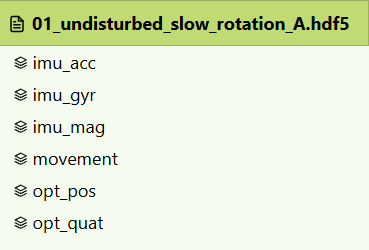
\includegraphics[width=\linewidth]{figures/dataset.png}
        \caption{Columns in the BROAD dataset}
        \label{fig:datase}
    \end{subfigure}
    \hfill
    \begin{subfigure}[t]{0.45\textwidth}
        \centering
        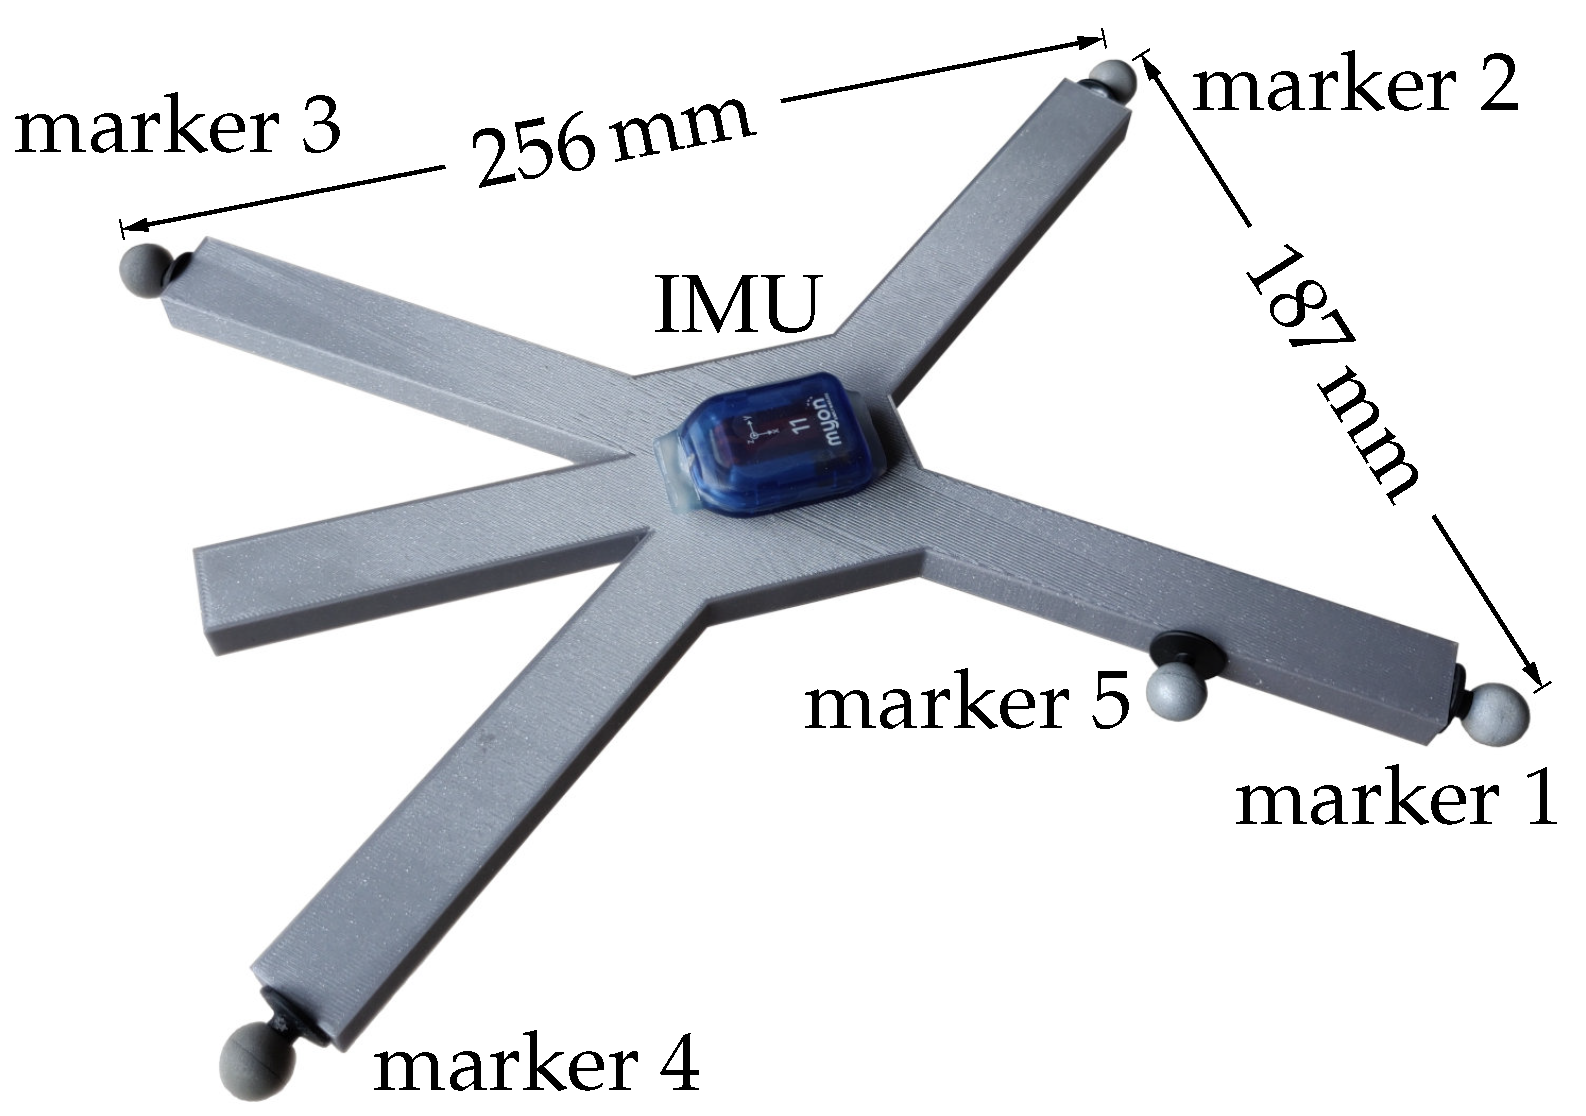
\includegraphics[width=\linewidth]{figures/imu_hardware_mount.png}
        \caption{3D printed hardware device with strapped on IMU.Optical markers placed on four corners for tracking}
        \label{fig:IMUhardware}
    \end{subfigure}
        
\end{figure}


\begin{algorithm} 
\caption{Modified CF algorithm} \label{CFalgo}
\DontPrintSemicolon
\SetAlgoLined
\SetAlgoNlRelativeSize{-1} % smaller line numbers
\SetNlSty{textbf}{(}{)}    % change line number style
\linespread{0.5}  

\KwIn{MARG sensor readings = $\{(g_1,a_1,m_1),(g_2,a_2,m_2),....\}$ , Toggling Engine , Noise Model , Alpha: $\alpha$, Duty Cycle Params: $d_l$ and $d_h$ }
\KwOut{Predicted gravity and north vectors $a_{pred}$ and $m_{pred}$}
\vspace{12pt}
Calibration sample count: $N=500$\\
Gyro bias: $g_{bias} = \sum_{i=0}^{N}g_i$ \\
Initial Gravity Vector Prediction: $a_{pred} = \sum_{i=0}^{N}a_i $ \\
Initial North Vector Prediction: $m_{pred} = \sum_{i=0}^{N}m_i $ \\
\vspace{12pt}
\ForEach{$(g_i,a_i,m_i)$ in MARG sensor Readings, $i>N$ \\}
{
Remove gyro bias and normalize accel-mag readings: 
\begin{align*}
    g_i&=g_i-g_{bias}\\
    a_i&=normalize(a_i)\\
    m_i&=normalize(m_i)
\end{align*}\\
Form $R_g$ from g_i.\\
Form the predictions from the gyro sensor:
\begin{align*}
a_{gyr} &= R_g\cdot a_{pred}\\
m_{gyr} &= R_g\cdot m_{pred}   
\end{align*}\\

Predict noise from noise model: $$(a_{noise},m_{noise}) = NoiseModel(g_i,a_i,m_i)$$\\
Predict alpha from the \textit{Toggling Engine}: $$\alpha = TogglingEngine(i,g_i,a_i,m_i)$$\\

Compute the dynamic scaling values:
\begin{align*}
e_{ga} &= \lVert \mathbf{a} - \mathbf{a}_g \rVert, &
e_{gm} &= \lVert \mathbf{m} - \mathbf{m}_g \rVert, &
e_{na} &= \lVert \mathbf{a}_{noise} \rVert, &
e_{nm} &= \lVert \mathbf{m}_{noise} \rVert \\
\alpha_{ga} &= \frac{\alpha \cdot e_{ga}}{e_{na} + e_{ga}}, &
\alpha_{gm} &= \frac{\alpha \cdot e_{gm}}{e_{nm} + e_{gm}}, &
\alpha_{na} &= \frac{e_{na}}{e_{na} + e_{ga}}, &
\alpha_{nm} &= \frac{e_{nm}}{e_{nm} + e_{gm}}
\end{align*}\\

Update the predictions:
\begin{align*}
    a_{pred} &= a_{gyr} - \alpha_{ga}(a_i - \alpha_{na}a_{noise} - a_{gyr}) \\
    m_{pred} &= m_{gyr} - \alpha_{gm}(m_i - \alpha_{nm}m_{noise} - m_{gyr})
\end{align*}\\

Normalize  the predictions:
\begin{align*}
    a_{pred} &= normalize(a_{gyr}) \\
    m_{pred} &= normalize(m_{gyr})
\end{align*}\\
Append $a_{pred}$ and $m_{pred}$ to $orientationEstimates$\\
}
\Return{$orientationEstimates$}
\end{algorithm}




\section{Gain($\alpha$) Estimation through Movement Prediction} \label{section:MovementPred}

Here we describe the working principle of the \textit{Toggling Engine}. The $\alpha$ parameter is initially set to be a constant value. The toggling engine is responsible for toggling the alpha in presence of movement. Detailed steps:
\begin{itemize}
    \item Train an XGBoost Classifier model\cite{chen2016xgboost} on the input features $X$ where $X$ contains the raw sensor readings of the MARG sensors and output class label $y$ where $y$ contains the boolean variable movement.
    \item Use the trained Model in the \textit{Toggling Engine} according to the \autoref{algo:toggling engine}.
\end{itemize}

\begin{algorithm}[H]
\SetAlgoLined
\DontPrintSemicolon
\KwIn{MARG Sensor Readings: $(g_i,a_i,m_i)$, Iteration Index $i$}
\KwData{Alpha: $\alpha$=0.01, Duty Cycle High: $d_h$, Duty Cycle Low: $d_l$,XGB Model $\mathcal{M}$}
\KwOut{Estimated $\alpha$}

\SetKwFunction{FMain}{TogglingEngine}
\SetKwProg{Fn}{Function}{:}{}

\Fn{\FMain{$i$,$g_i$,$a_i$,$m_i$}}{
    Compute total period: $T \gets d_h + d_l$\;
    Predict movement: $\hat{\delta} \gets \mathcal{M}(g_i,a_i,m_i)$\;

    \uIf{$\hat{\delta} == 0$}{
         \KwRet{$\alpha$}
    }
    
    \uIf{$(i \bmod T) < d_h$}{
        $\alpha \gets \alpha $
    }
    \Else{
        $\alpha \gets 0$ 
    }

    \KwRet{$\alpha$}
}
\caption{Toggling Engine} \label{algo:toggling engine}
\end{algorithm}

\section{Noise Removal} \label{section:noise_removal}
Here we describe the training procedure of the model that removes noise. The ground truth noise values are established from the difference of actual sensor measurements and the ground truth gravitational and magnetic north vectors. The ground truth quaternion $q_{gt}$ generated from the quaternion components in \texttt{opt\_quat} in the dataset is used to rotate the $a_{avg}$ and $m_avg$ vectors to remove the noises. The $a_{avg}$ and $m_avg$ vectors are calculated by averaging initial sensor readings for $N=500$ iterations. The value of $N$ could be varied.
\begin{itemize}
    \item Ground truth gravity vector is calculated using the ground  truth $q_{gt}$ obtained for each record in a recording dataset \texttt{opt\_quat}:
    More information on this rotation formula in \autoref{subsec:rotatevector}
    \begin{equation} \label{eqn:acc noise removal} 
        a_{gt} = q_{gt}^{-1} \cdot a_{avg} \cdot q_{gt}
    \end{equation}
    \item Ground truth magnetometer north vector is calculated using the ground  truth $q_{gt}$ obtained for each record in a recording dataset \texttt{opt\_quat}:
    \begin{equation} \label{eqn:mag noise removal}
        m_{gt} = q_{gt}^{-1} \cdot m_{avg} \cdot q_{gt}
    \end{equation}
    \item An XGBoost Regression model\cite{chen2016xgboost} is to be trained with input features $X$ being the raw MARG sensor readings and the output feature $y$ being the six components of the $a_{gt}$ and $m_{gt}$ vectors. The training dataset contains may contain all the MARG sensor readings from all the recordings, each sensor reading corresponds to a ground truth quaternion $q_{gt}$ represented as \texttt{opt\_quat} in the datasets. Each of the $q_{gt}$ is used to generate $a_{gt}$ and $m_{gt}$ vectors used for the regression model training. The loss function used is the generic \textit{Mean Squared Error Loss function} \cite{bickel2015mathematical}. The trained model is to be used to do noise prediction in \autoref{CFalgo} where the noise is subtracted from the sensor readings.
\end{itemize}

\chapter{Experimental Setup} \label{chapter:setup}

\section{Mechanical Platform (Turntable)}

\subsection{Turntable Setup}

The experimental turntable was designed in Fusion360 as shown in \autoref{fig:turntable_fusion} and constructed using 3D-printed parts and integrated sensors 
to provide both actuation and ground-truth angle measurement. The constructed device is shown in \autoref{fig:real turntable} and \autoref{fig:no disk}. 
The system consists of a circular rotating disk mounted on a bearing, 
a box-shaped support structure, and a base platform with a magnet for the AS5600 magnetic encoder. 
The disk carries the electronics, including a Raspberry Pi 5, an MPU9250 MARG sensor, and a 20,000\,mAh power bank, 
which provides standalone operation. The detailed specifications of the turntable are summarized below.

\begin{itemize}
    \item \textbf{Turntable geometry:} Diameter [XX\,cm], 3D printed PLA/ABS material, mass [YY\,g].
    \item \textbf{Actuation:} There is no electrical actuation built into the turntable, rather movement is executed by manually rotating the turntable.
    \item \textbf{Mechanical construction:} 
    \begin{itemize}
        \item Upper circular disk connected to the inner ring of the 6010 bearing.
        \item Box-shaped 3D printed housing supporting the bearing.
        \item Platform with embedded magnet for AS5600 encoder.
    \end{itemize}
    \item \textbf{Ground-truth sensing:} \textbf{Ground-truth sensing:} AS5600 absolute magnetic encoder with the following characteristics:
        \begin{itemize}
        \item Resolution: 12-bit (4096 positions per revolution, $\approx 0.087^{\circ}$ per step).
        \item Angular accuracy: typically $\pm 0.5^{\circ}$ to $\pm 1^{\circ}$, depending on magnet alignment and air gap.
        \item Maximum angular deviation: up to $\pm 1.4^{\circ}$ worst-case under misalignment or offset conditions.
        \item Latency: on the order of 1–2\,ms (limited by I$^2$C polling rate or PWM readout frequency).
        \item Output interfaces: I$^2$C, PWM, or analog voltage.
        \end{itemize}    \item \textbf{On-disk payload:} 20,000\,mAh powerbank, Raspberry Pi 5 (8\,GB), MPU9250 MARG sensor, AS5600 encoder.
\end{itemize}


\subsection{Electronics & Sensors}
The inertial sensing subsystem is based on the InvenSense/TDK MPU-9250, which integrates a tri-axial accelerometer, gyroscope, and the AK8963 tri-axial magnetometer. Each sensing axis employs 16-bit ADCs, ensuring adequate dynamic range for motion tracking. The IMU was mounted on a 3D-printed cube positioned at the edge of the turntable disk. Directly beneath the ring connecting the disk to the bearing, the AS5600 magnetic angle encoder was fixed, enabling precise alignment between inertial measurements and ground-truth angular position.

\begin{itemize}
  \item \textbf{IMU:} InvenSense/TDK MPU-9250, tri-axial accelerometer and gyroscope with integrated AK8963 magnetometer, 16-bit ADCs.
  \item \textbf{Gyroscope ranges:} $\pm$250, $\pm$500, $\pm$1000, and $\pm$2000 dps (default range used).
  \item \textbf{Accelerometer ranges:} $\pm$2, $\pm$4, $\pm$8, and $\pm$16 g (default range used).
  \item \textbf{Sample-rate and DLPF settings:} Default sample rate and default digital low-pass filter configuration were used.
  \item \textbf{Processor/DAQ:} Raspberry Pi 5 (8 GB) running the default Raspberry Pi OS. Communication with both the MPU-9250 and the AS5600 magnetic encoder was established over 
                                the I$^2$C bus. Supply voltage and logic level were 3.3 V.
  \item \textbf{Power:} A 20,000 mAh USB power bank mounted on the disk provided power to the Raspberry Pi, IMU, and encoder.
\end{itemize}


\subsection{Motion Protocols}

The turntable experiments were conducted under three categories of motion: static, quasi-static, and dynamic. The coordinate frames tested were determined by the feasible orientations of the setup: rotation was applied around the $z$-axis and $y$-axis with the positive direction pointing upward, and around the $x$-axis with the positive direction pointing downward. Rotation around the $x$-axis upward was not performed due to mechanical constraints imposed by wiring. The three types of motions are described below:
\begin{itemize}
    \item \textbf{Static:} The system experiences no movement. This condition is used to establish baseline sensor stability and drift characteristics.
    
    \item \textbf{Quasi-static:} Slow and controlled movements are applied, typically at speeds low enough that inertial effects are negligible. This allows the evaluation of sensor accuracy under gradual angular changes.
    
    \item \textbf{Dynamic:} Continuous and rapid motions are applied, where inertial effects are significant. This tests the system response under sustained rotation and higher angular velocities.
\end{itemize}

\subsection{Software Setup and Result Generation}

The software infrastructure for the experimental turntable was implemented on a Raspberry Pi 5 (8\,GB). The system executes four independent Python scripts corresponding to different orientation estimation algorithms: the proposed filter, the AQUA filter, the Extended Kalman Filter (EKF), and the Madgwick filter. These scripts are coordinated by a parent \texttt{run} script, which launches each of the four filter scripts in separate threads to allow concurrent execution.

Each filter script reads sensor measurements from the MPU-9250 MARG sensor via the I$^2$C protocol, capturing tri-axial accelerometer, gyroscope, and magnetometer data. In parallel, a dedicated script reads angle measurements from the AS5600 magnetic encoder and converts the encoder readings into a ground-truth quaternion representation of the turntable orientation.

During runtime, the estimated quaternions from the four filters, along with the ground-truth quaternion, are continuously recorded into CSV files. Post-processing involves computing the quaternion absolute distance metric as in \autoref{appendix:quaternion-distance}, between the ground-truth quaternion and each filter's estimate. These distance metrics are then plotted to visualize and compare the performance of the different orientation filters under various motion conditions. The summarized version
of the results are shown in \autoref{section:mechanical_platform_result}. The graphs of the results can be found in the appendix. 


\begin{figure}[h!]
    \centering
    \begin{subfigure}[b]{0.3\textwidth}
        \centering
        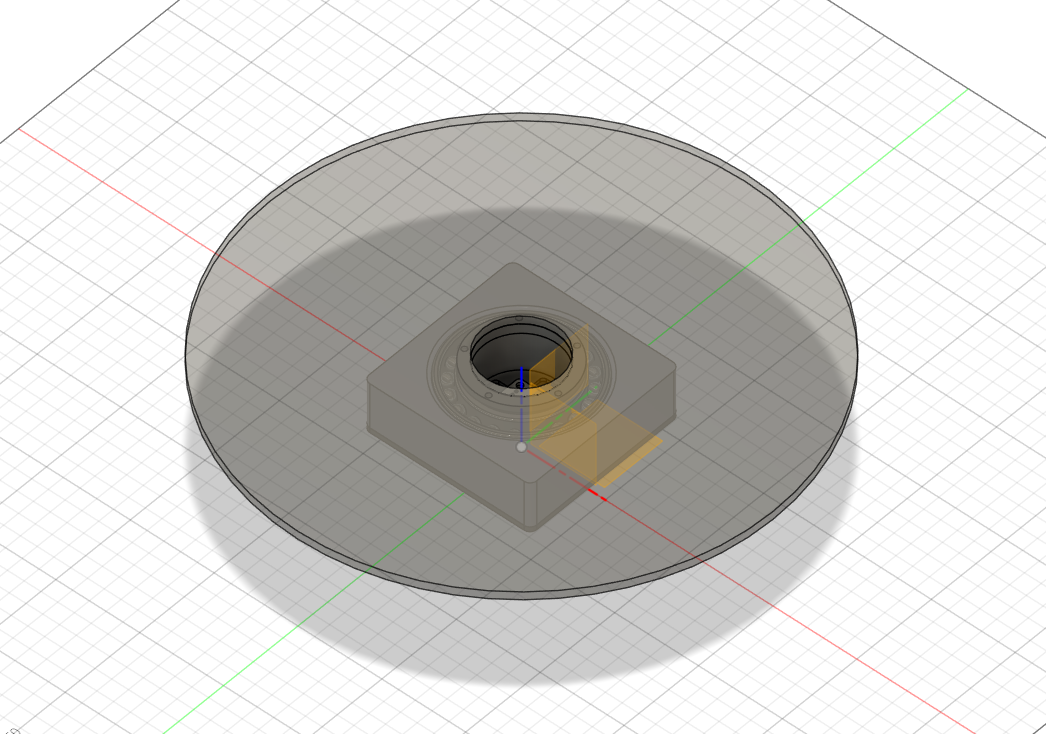
\includegraphics[width=\textwidth]{Turntable_fusion.png}
        \caption{Fusion360 model of the turntable}
        \label{fig:turntable_fusion}
    \end{subfigure}
    \hfill
    \begin{subfigure}[b]{0.3\textwidth}
        \centering
        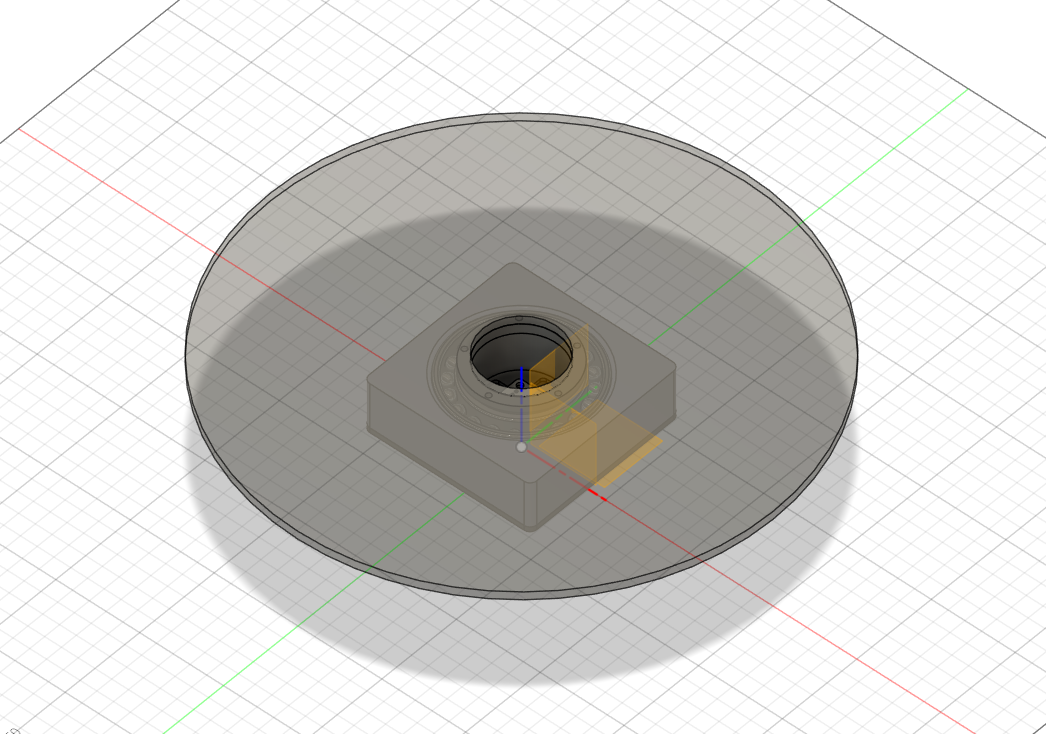
\includegraphics[width=\textwidth]{Turntable_fusion.png}
        \caption{Actual Constructed Turntable}
        \label{fig:real turntable}
    \end{subfigure}
    \hfill
    \begin{subfigure}[b]{0.3\textwidth}
        \centering
        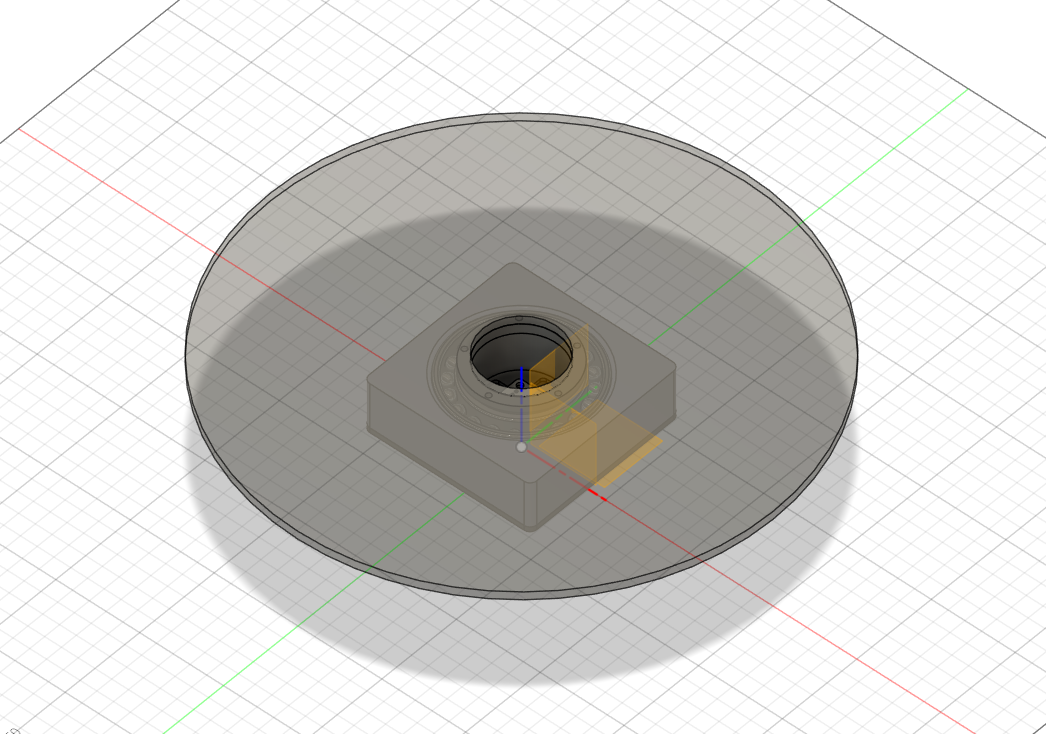
\includegraphics[width=\textwidth]{Turntable_fusion.png}
        \caption{With the disk Removed}
        \label{fig:no disk}
    \end{subfigure}
    \caption{Overview of the turntable setup with key components highlighted.}
    \label{fig:turntable_overview}
\end{figure}


\begin{table}[h!]
\centering
\caption{Summary of motion protocols applied to the turntable}
    \begin{tabular}{|c|p{10cm}|}
    \hline
    \textbf{Motion Type} & \textbf{Description} \\
    \hline
    Static & No movement; turntable held stationary. \\
    \hline
    Quasi-static & Rotation from $0^{\circ}$ to $180^{\circ}$ clockwise, then $0^{\circ}$ to $180^{\circ}$ counterclockwise; break; repeated once (total of two cycles). \\
    \hline
    Dynamic & Continuous full rotations: 3 turns, break, 4 turns, break, 5 turns. \\
    \hline
    \end{tabular}
\end{table}


\section{Datasets}
The dataset was already presented in \autoref{section:dataset}. Based on this the experimental pipeline was generated. The experiment is carried out in 3 parts, in the initial two parts the models for the movement and noise prediction are trained on the BROAD\cite{BROAD} dataset. Then the trained model is used to implement the Modified CF as of \autoref{CFalgo} and the results are reported as absolute distance between the Ground truth and the predicted rotation quaternions\cite{absoluteDistance}.



\subsection{Training to Predict Movement}
In this part we discuss the training process of the XGBoost Classifier model to predict movement. The detailed steps:
\begin{itemize}
    \item BROAD dataset has 39 recordings. All the 39 recordings are concatenated one after another and a concatenated dataset containing all records from 39 recordings are formed. The setup for input features \verb|X| and the output feature \verb|y| goes as: \\
    \begin{table}[htbp]
    \centering
    \caption{Dataset Generation to Predict Movement}    \label{tab:sensor_readings}
        \begin{adjustbox}{max width=0.8\textwidth}
            \begin{tabular}{| p{0.45\textwidth} | p{0.45\textwidth} |}
            \hline
            \textbf{X} & \textbf{y} \\
            \hline
            All records/samples of MARG sensor readings from the concatenated dataset & Corresponding movement column of the concatenated dataset \\
            \hline
            \end{tabular}
        \end{adjustbox}
    \end{table}
    After forming X and y the datasets were split to train and test sets with train set having 20\% of the split.

    \item After the formation of \texttt{X} and \texttt{y}, we train an XGBoost Classifier model optimized through the \verb|Oputna Study| library\cite{akiba2019optuna}.The optuna study was constructed to maximize the \texttt{accuracy\_score}\cite{labatut2012accuracy} among the \texttt{y\_test} and the predicted \texttt{y\_pred}. The suggested parameters for the \textit{study} were chosen as in \autoref{tab:xgb_hyperparameters_movement}:
    \begin{table}[htbp]
    \centering
    \caption{Choice of Ranges of Hyperparams for \textit{Optuna Study(For Movement)} }
    \label{tab:xgb_hyperparameters_movement}
        \begin{tabular}{|l|l|l|}
        \hline
            \textbf{Hyperparameter} & \textbf{Description} & \textbf{Range} \\ \hline
            \texttt{colsample\_bytree} & Fraction of features to sample per tree. & [0.0, 1.0] \\ \hline
            \texttt{learning\_rate} & Step size shrinkage to prevent overfitting. & [0.0, 1.0] \\ \hline
            \texttt{max\_depth} & Maximum depth of a tree. & [2, 15] \\ \hline
            \texttt{n\_estimators} & Number of boosting rounds. & [1, 15] \\ \hline
            \texttt{reg\_alpha} & L1 regularization term on weights. & [0, 10] \\ \hline
            \texttt{reg\_lambda} & L2 regularization term on weights. & [0, 10] \\ \hline
            \texttt{subsample} & Fraction of samples to use per tree. & [0.6, 1.0] \\ \hline
        \end{tabular}
    \end{table}

    \item After running the Optuna Study for \texttt{N=100} iterations, the best hyperparameter was chosen and 
    the model was trained choosing the best hyperparams.
\end{itemize}

\subsection{Training to Predict Noise} \label{subsec:predictnoise}
This subsection focuses on the training of model to predict the noises among the reported sensor readings. Detailed steps:
\begin{itemize}
    \item There are 39 recordings in the dataset of BROAD. We choose the recordings \texttt{concat\_list=[0,1,2,3,4,5,6,7,9,10,11,12,13,15,16,18,19,20,21,23, \\ 24,25,26,27,28,29,31,32,33,34,35,36,37,38]}.
    
    \item For each recording in \texttt{concat\_list} we follow the procedure mentioned in \autoref{section:noise_removal}. We average the first $N$ entries then generate \texttt{a\_noise} according to \autoref{eqn:acc noise removal} and \texttt{m\_noise} according to \autoref{eqn:mag noise removal} for each record \texttt{i}. Then generate a new .csv dataset for each recording whose columns contain 9 MARG sensor raw values and 6 noise values ( 3 component from \texttt{a\_noise} and 3 component from \texttt{m\_noise}. Doing it for each recording in \texttt{concat\_list} generates 34 new csv datasets. We concatenate all of them to form a large dataset.
    \item Generate \texttt{X} and \texttt{y} from the large dataset according to \autoref{tab:noisevals}
        \begin{table}[H]
        \centering
        \caption{Dataset Generation to Predict Noise}    \label{tab:noisevals}
            \begin{adjustbox}{max width=0.8\textwidth}
                \begin{tabular}{| p{0.45\textwidth} | p{0.45\textwidth} |}
                \hline
                \textbf{X} & \textbf{y} \\
                \hline
                All records/samples of MARG sensor readings from the concatenated dataset & Corresponding 6 values of a\_noise and m\_noise \\
                \hline
                \end{tabular}
            \end{adjustbox}
        \end{table}
    
    \item Choice of model was \textbf{XGB regressor} but coupled with the \textbf{Random Sample Consensus(RANSAC)}\cite{fischler1981random} algorithm. The ransac algorithm made training the base XGB regressor more robust to outliers and it improved the bias variance tradeoff.
    
    \item Split the dataset into train and test sets. Generate an optuna study\cite{akiba2019optuna} where the model is trained 
    within the study objective on the train set and the objective works to maximize the r2\_score on the test set. The choice of hyperparameters is the same as in \autoref{tab:xgb_ransac_hyperparams}. The study runs for 200 iterations.
    \begin{table}[H]
    \centering
    \caption{Hyperparameter Search Space for XGBoost Regressor with RANSAC}
    \label{tab:xgb_ransac_hyperparams}

        \begin{adjustbox}{max width=0.7\textwidth}
            \begin{tabular}{|l|c|c|p{0.3\textwidth}|}
                \hline
                \textbf{Hyperparameter} & \textbf{Type} & \textbf{Range} & \textbf{Description} \\
                \hline
                \texttt{colsample\_bytree} & Float & [0.0, 1.0] & Subsample ratio of columns for each tree \\
                \texttt{learning\_rate} & Float & [0.0, 1.0] & Step size shrinkage used in update to prevent overfitting \\
                \texttt{max\_depth} & Integer & [2, 15] & Maximum depth of a tree \\
                \texttt{n\_estimators} & Integer & [1, 25] & Number of boosting rounds \\
                \texttt{reg\_alpha} & Float & [0.0, 10.0] & L1 regularization term on weights \\
                \texttt{reg\_lambda} & Float & [0.0, 10.0] & L2 regularization term on weights \\
                \texttt{subsample} & Float & [0.6, 1.0] & Subsample ratio of the training instances \\
                \texttt{min\_samples} & Float & [0.1, 0.9] & Minimum number of samples for a model to be considered valid in RANSAC \\
                \texttt{residual\_threshold} & Float & [1e-3, 10.0] & Maximum residual for a data point to be classified as an inlier in RANSAC \\
                \texttt{max\_trials} & Integer & [100, 500] & Maximum number of iterations for RANSAC algorithm \\
                \hline
            \end{tabular}          
        \end{adjustbox}
    \end{table}
    

    
    \item The final model is trained with the best hyper parameter returned from the \texttt{study} object.

\end{itemize}
\subsection{Implementation and Testing of the Modified Complementary Filter} \label{section:impl-and-testing}
The complementary filter with all its modifications proposed in \autoref{CFalgo} were implemented using \texttt{python}. Separate classes were constructed for the \textit{Toggling Engine} and \textit{Complementary Filter} implementation. Code of the actual implementaion could be found \href{https://github.com/azfarus/NDAG_MARG_THESIS_v2}{here}.
\par
After implementation, the filter was fed with sensor readings from  \texttt{cv\_set=[8, 14, 17, 22, 30]}\label{cv_set} where each indexes correspond to the index of the recording file not in the \texttt{train\_set}.The \texttt{cv\_set} is being used for cross-validation. Each of the recording file fed through the filter gave us a quaternion estimation for each iteration, i.e. the file \texttt{01\_undisturbed\_slow\_rotation\_A} has approximately 56,000 sensor readings. Each sensor reading will correspond to a quaternion estimation($q_{esti}$) and a ground truth($q_{gti}$) quaternion. The error metric per iteration stands to be:
\begin{equation}
    e_i = Quat_{abs\_dist}(q_{gti},q_{esti})
\end{equation}
More information about the metric is provided in \autoref{appendix:quaternion-distance}. We compare the mean of all $e_i$ found over a particular recording for various standard filters such as the Madgwick and the Complementary filter to our proposed filter.






\chapter{Results} \label{chapter:results}



\section{Results of noise Prediction}
The XGB regression model run according to \autoref{subsec:predictnoise} showed promising result in being able to predict the amount of noise in test set. The test set contained the recordings with indexes \texttt{cv\_set=[8, 14, 17, 22, 30]}. The summary of the result is showed in \autoref{tab:xgb_ransac_results_hyperparam}. The r2 scores are reported for the \texttt{cv\_set} and the test set generated after \texttt{train\_test\_split}.
\begin{table}[htbp]
\centering
\caption{Final Hyperparameters for XGB RANSAC and Model Evaluation Results}
\label{tab:xgb_ransac_results_hyperparam}
\begin{tabular}{|l|c||l|c|}
    \hline
        \multicolumn{2}{|c||}{\textbf{Hyperparameters}} & \multicolumn{2}{c|}{\textbf{Test Results}} \\
        \hline
        \texttt{degree} & 2 & \texttt{R\textsuperscript{2} Score Test Set} & 0.8893 \\
        \texttt{colsample\_bytree} & 0.9274 &  & \\
        \texttt{learning\_rate} & 0.3028 & & \\
        \texttt{max\_depth} & 15 & & \\
        \texttt{n\_estimators} & 20 & & \\
        \texttt{reg\_alpha} & 0.1242 & \texttt{R\textsuperscript{2} Score CV Set} & 0.620 \\
        \texttt{reg\_lambda} & 0.7352 & & \\
        \texttt{subsample} & 0.6777 & & \\
        \texttt{min\_samples} & 0.2392 & & \\
        \texttt{residual\_threshold} & 5.0912 & & \\
        \texttt{max\_trials} & 136 & & \\
        \hline
    \end{tabular}
\end{table}

\section{Results of Movement Prediction}

The XGB Classifier model run according to \autoref{section:MovementPred} showed promising result in being accurate about prediction the movement. The training set contained all the recordings from 1 to 39. The summary of the result is showed in \autoref{tab:xgb_movement_results_hyperparam}. The accuracy score is reported for the maximum accuracy acheived in the trial conducted by \texttt{Optuna Study}. The metric used for this is the \texttt{accuracy\_score}\cite{labatut2012accuracy}.
\begin{table}[htbp]
\centering
\caption{Final Hyperparameters for Movement Prediction XGB Classfier}
\label{tab:xgb_movement_results_hyperparam}
\begin{tabular}{|l|c||p{0.3\textwidth}|c|}
    \hline
        \multicolumn{2}{|c||}{\textbf{Hyperparameters}} & \multicolumn{2}{c|}{\textbf{Test Results}} \\
        \hline
        \texttt{degree} & 1 &  &  \\
        \texttt{colsample\_bytree} & 0.9382 &  & \\
        \texttt{learning\_rate} & 0.6043 & & \\
        \texttt{max\_depth} & 15 & & \\
        \texttt{n\_estimators} & 22 & & \\
        \texttt{reg\_alpha} & 2.02025 & \texttt{Movement Prediction accuracy over the test split} & 0.996 \\
        \texttt{reg\_lambda} & 2.8650 & & \\
        \texttt{subsample} & 0.9198 & & \\
        \texttt{min\_samples} & 0.7556 & & \\
        \texttt{residual\_threshold} & 2.3906 & & \\
        \texttt{max\_trials} & 136 & & \\
        \hline
    \end{tabular}
\end{table}


\section{Performance of Our Filter on BROAD Dataset Vs Standard Implementations}

The experimental setup was implemented following the steps mentioned in \autoref{section:impl-and-testing}. The \texttt{cv\_set} contains \texttt{[8, 14, 17, 22, 30]} file indexes. Thus results were generated based on these 5 files where noise removal was done. Results for simply performing toggling was evaluated over all the 39 recordings.

\subsection{Results with only Toggling Engine, no noise Removal}
In this subsection the charts of Mean errors and Error variance have been shown in \autoref{result:meanerrortoggle} and \autoref{result:varerrortoggle} respectively. These charts were generated from the implementation of \autoref{CFalgo} but without the noise prediction model removing the noise from the sensor readings. The duty cycle chosen was 50\% and $\alpha$ was chosen a low value of \texttt{0.001}. 

\begin{figure}[H]
    \centering
    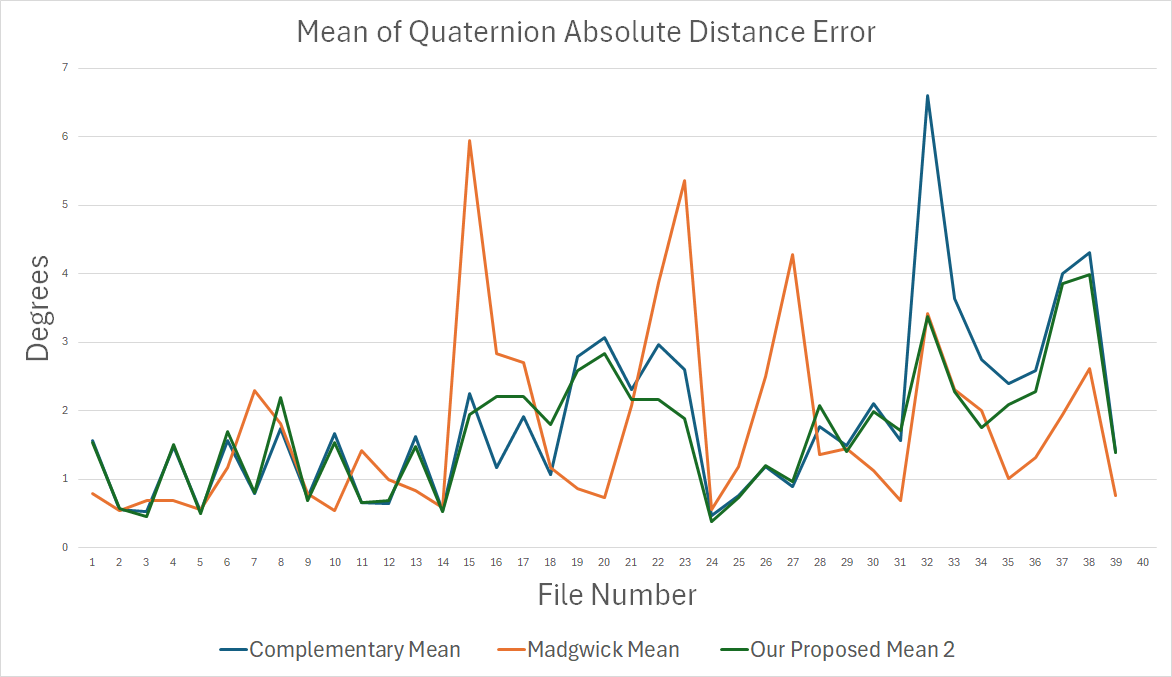
\includegraphics[width=0.9\linewidth]{figures/mean_for_39_files.png}
    \caption{Mean of errors on all 39 recordings, for the Madgwick, Complementary , and our Complementary filtering with movement prediction and toggling with 50\% duty cycle}
    \label{result:meanerrortoggle}
\end{figure}

\begin{figure}[H]
    \centering
    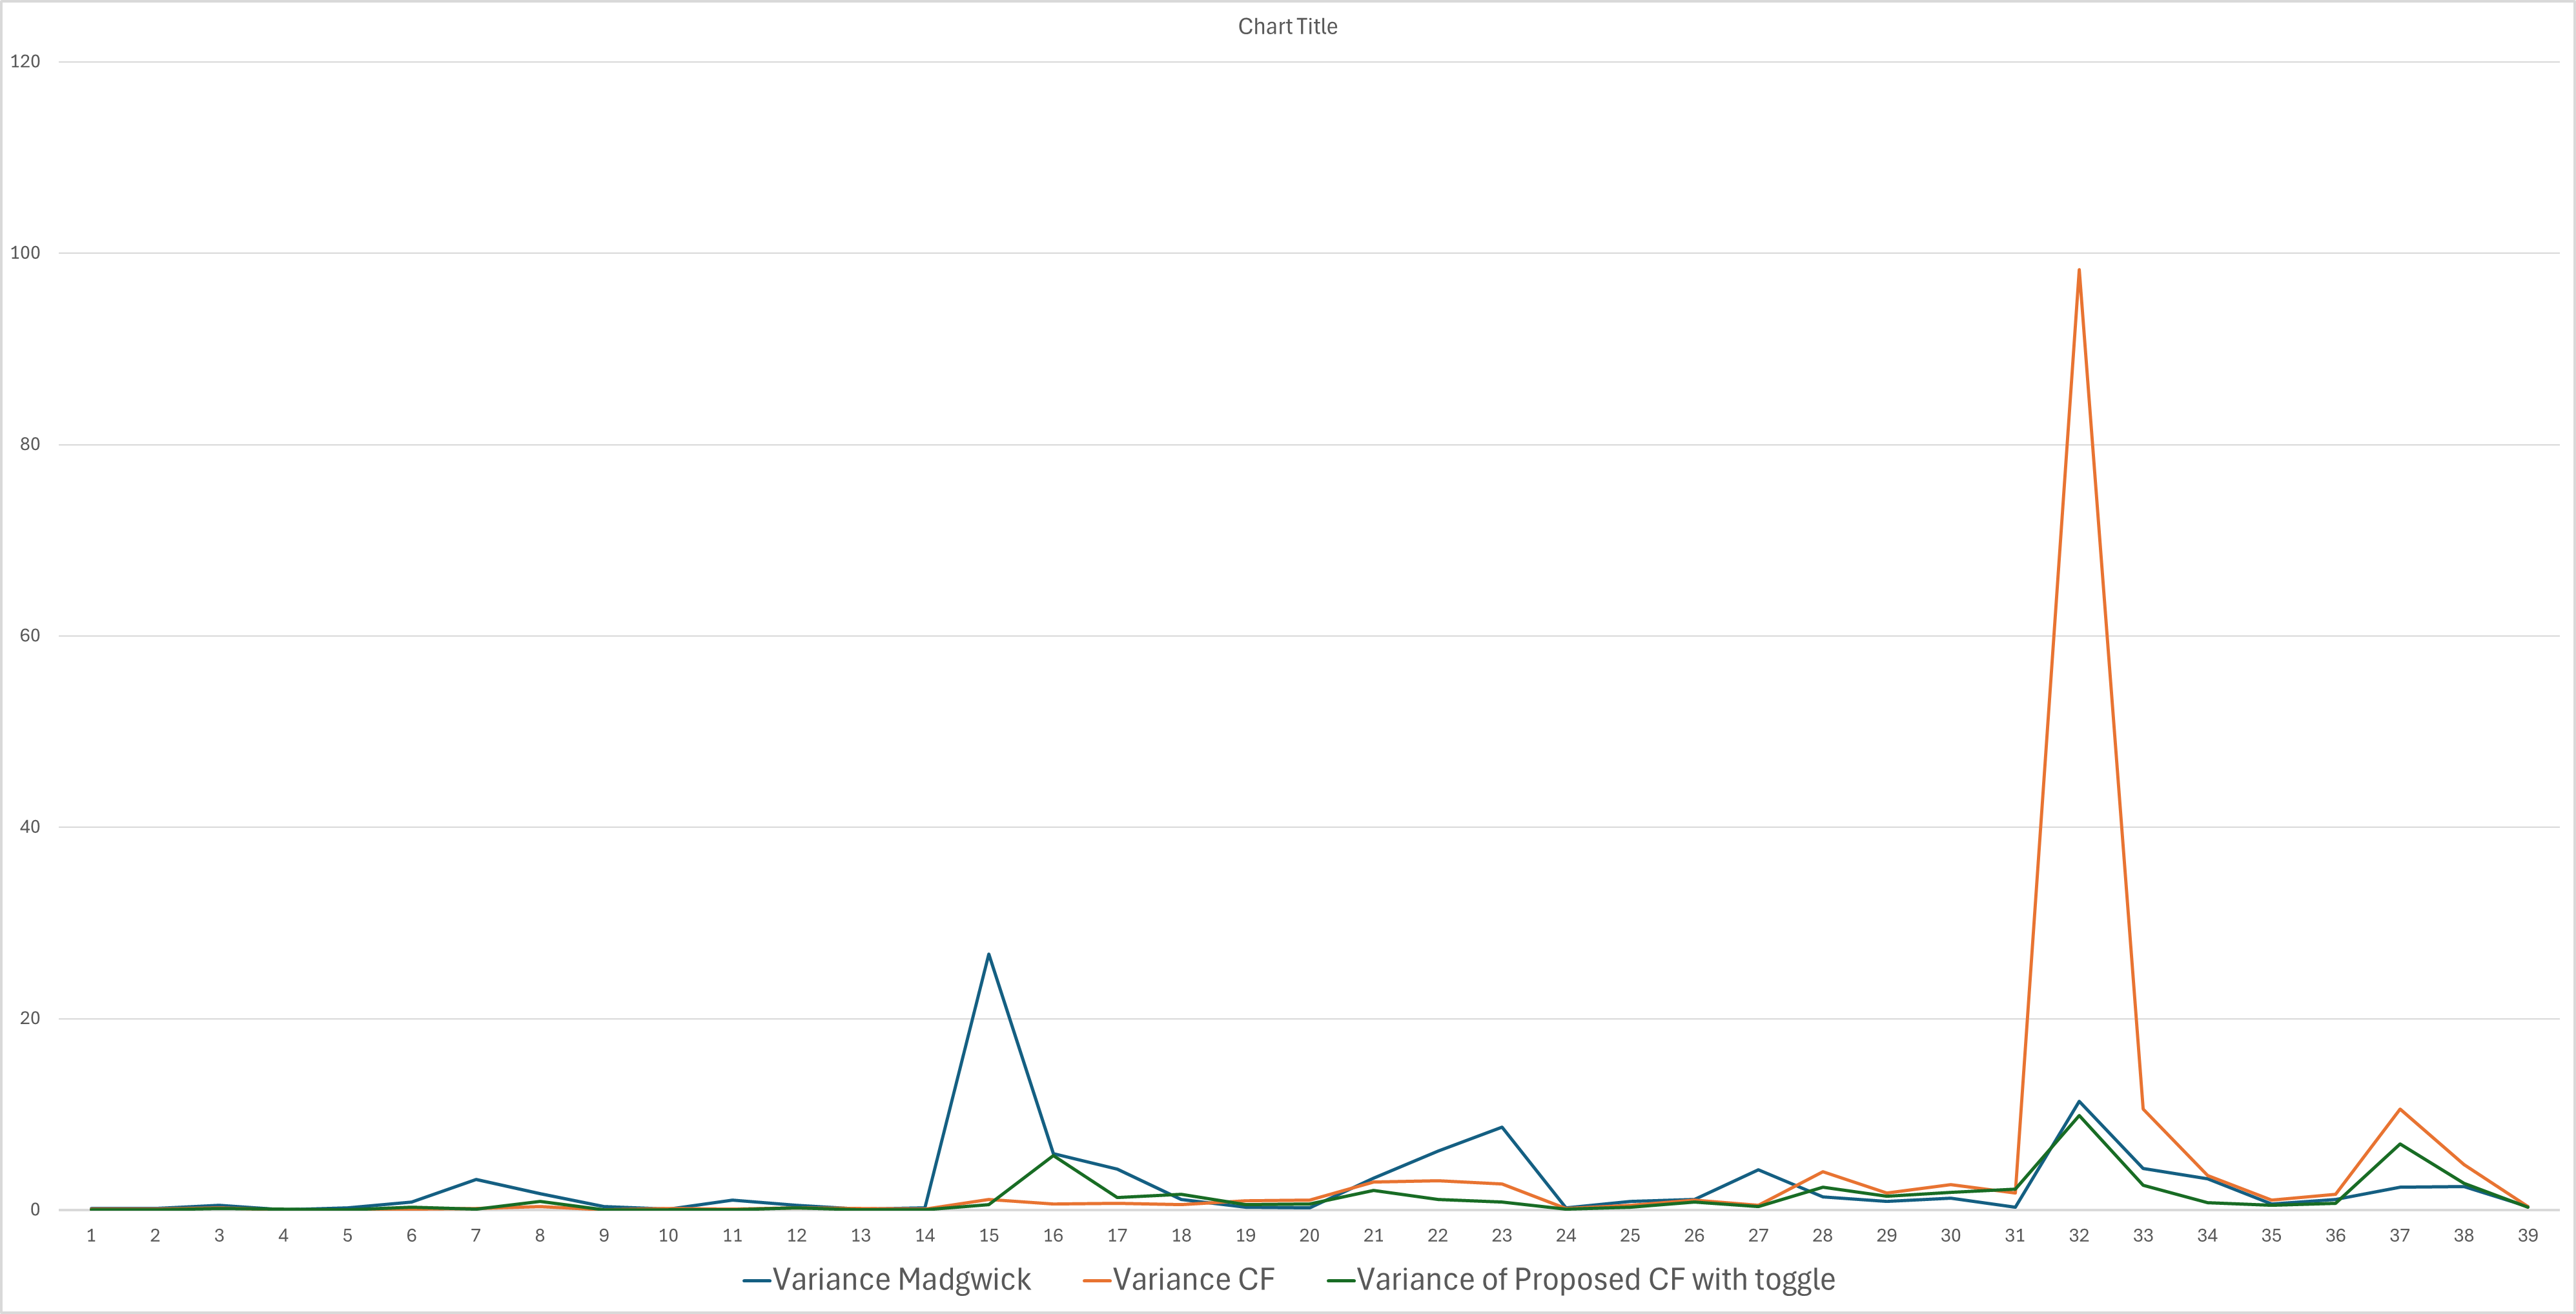
\includegraphics[width=1\linewidth]{figures/variance_toggle.png}
    \caption{Variance of errors on all 39 recordings, for the Madgwick, Complementary , and our Complementary filtering with movement prediction and toggling with 50\% duty cycle}
    \label{result:varerrortoggle}
\end{figure}

\subsection{Results of CF with $\alpha$-toggling and Noise removal}
This subsection displays the result of $\alpha$-toggling noise removing Complementary filter which is the complete realization of \autoref{CFalgo}. The charts only compare the results on 5 files of the \texttt{cv\_set} containing \texttt{[8, 14, 17, 22, 30]}, as the other files were used to train the noise removal model. The mean and variance results are shown in \autoref{tab:error_statistics_cvset_mean} and \autoref{tab:error_statistics_cvset_variance} respectively. The chart in \autoref{fig:chart_rmnoise_comparison} shows a comparision between the noise removal approach with other filters.

\begin{table}[H]
\centering
\caption{Mean Error Statistics across the \texttt{cv\_set}}
\label{tab:error_statistics_cvset_mean}
    \begin{tabular}{|p{0.3\textwidth}|p{0.2\textwidth}|p{0.2\textwidth}|p{0.2\textwidth}|}
    \hline
    \textbf{Filename} & \textbf{Basic CF} & \textbf{Proposed CF} & \textbf{ MadgWick Filter} \\
    \hline
    09 undisturbed fast rotation with breaks B.hdf5 & 0.8134 & 0.7408 & 0.7899 \\
    \hline
    15 undisturbed fast translation A.hdf5 & 3.1007 & 1.6212 & 5.9503 \\
    \hline
    18 undisturbed fast translation with breaks B.hdf5 & 5.5009 & 1.2757 & 1.1728 \\
    \hline
    23 undisturbed fast combined 360s.hdf5 & 3.6085 & 2.7388 & 5.3682 \\
    \hline
    31 disturbed stationary magnet D.hdf5 & 2.4708 & 1.5798 & 0.6953 \\
    \hline
    \end{tabular}
\end{table}

\begin{table}[H]
\centering
\caption{Variance of Error Statistics across the \texttt{cv\_set}}
\label{tab:error_statistics_cvset_variance}
    \begin{tabular}{|p{0.3\textwidth}|p{0.2\textwidth}|p{0.2\textwidth}|p{0.2\textwidth}|}
    \hline
    \textbf{Filename} & \textbf{Basic CF} & \textbf{Proposed CF} & \textbf{MadgWick Filter} \\
    \hline
    09 undisturbed fast rotation with breaks B.hdf5 & 0.1110 & 0.2603 & 0.3510 \\
    \hline
    15 undisturbed fast translation A.hdf5 & 3.8544 & 0.9997 & 26.7320 \\
    \hline
    18 undisturbed fast translation with breaks B.hdf5 & 31.1229 & 1.1998 & 1.1499 \\
    \hline
    23 undisturbed fast combined 360s.hdf5 & 2.8928 & 1.1746 & 8.7074 \\
    \hline
    31 disturbed stationary magnet D.hdf5 & 4.9321 & 1.5576 & 0.3195 \\
    \hline
    \end{tabular}
\end{table}

\begin{figure}[H]
    \centering
    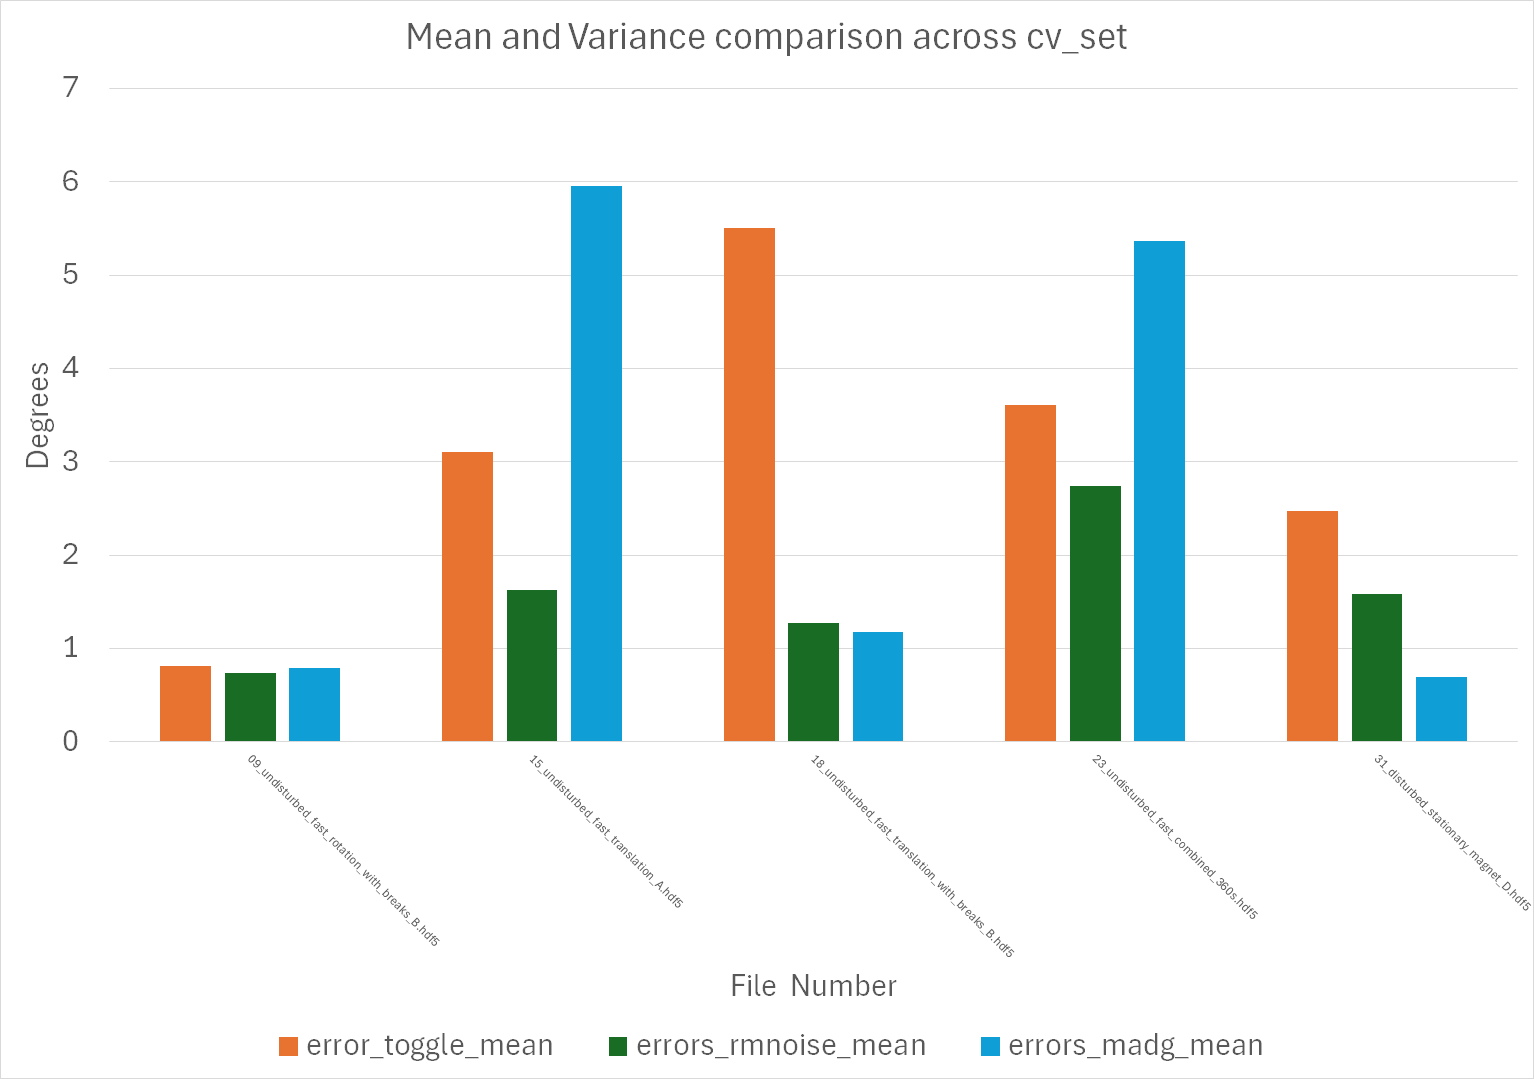
\includegraphics[width=0.75\linewidth]{figures/rmnoise_chart.png}
    \caption{Mean and Variance comparison across cv\_set. Filenames are sequentially arranged according to \autoref{tab:error_statistics_cvset_mean}}
    \label{fig:chart_rmnoise_comparison}
\end{figure}


\subsection{Results of CF with $\alpha$-Toggling and Noise Removal on Individual Files} \label{subsec:individualFiles}
This subsection illustrates the performance of the filter on a particular recording of the BROAD dataset over the iterations. Before demonstration of the graphs, the process how the error graphs on individual files have been generated should be stated.
\begin{itemize}
    \item The individual record files have 50,000 to 300,000 sensor readings. Each reading correspond to a Quaternion Estimate $q_{esti}$.
    \item Each reading also corresponds to a ground truth quaternion $q_{gti}$.
    \item Their distance is calculated according to the process mentioned in \autoref{section:impl-and-testing}.
    \item This distance/error is plotted vs the iteration count in figures \ref{fig:9_undisturbed_fast_rotation_with_breaks_B},\ref{fig:15_undisturbed_fast_translation_A},\ref{fig:18_undisturbed_fast_translation_with_breaks_B},\ref{fig:23_undisturbed_fast_combined_360s} and \ref{fig:31_disturbed_stationary_magnet_D}.
    \item \textbf{Legend:}
    \begin{itemize}
        \item \textit{\textbf{Red:}} Madgwick Filter
        \item \textit{\textbf{Green:}} Complementary Filter
        \item \textit{\textbf{Blue:}} Our Proposed Filter
    \end{itemize}
\end{itemize}

\begin{figure}[H]
    \centering
    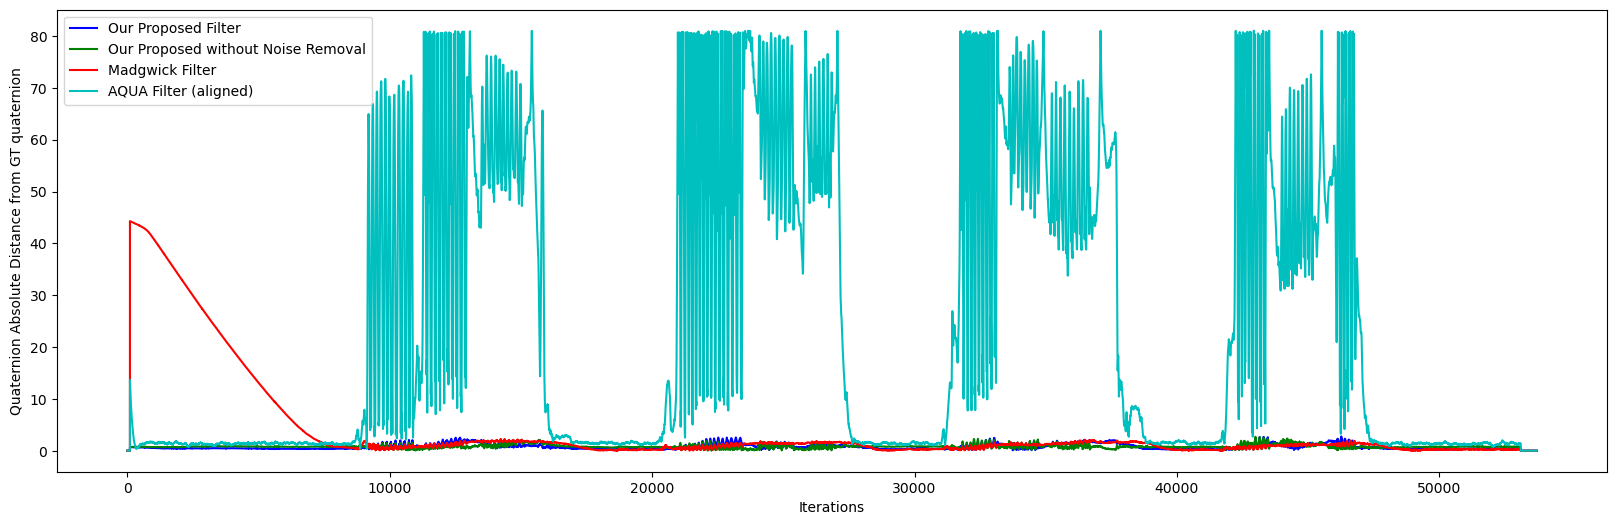
\includegraphics[width=0.9\linewidth]{figures/9_undisturbed_fast_rotation_with_breaks_B.png}
    \caption{9\_undisturbed\_fast\_rotation\_with\_breaks\_B}
    \label{fig:9_undisturbed_fast_rotation_with_breaks_B}
\end{figure}

\begin{figure}[H]
    \centering
    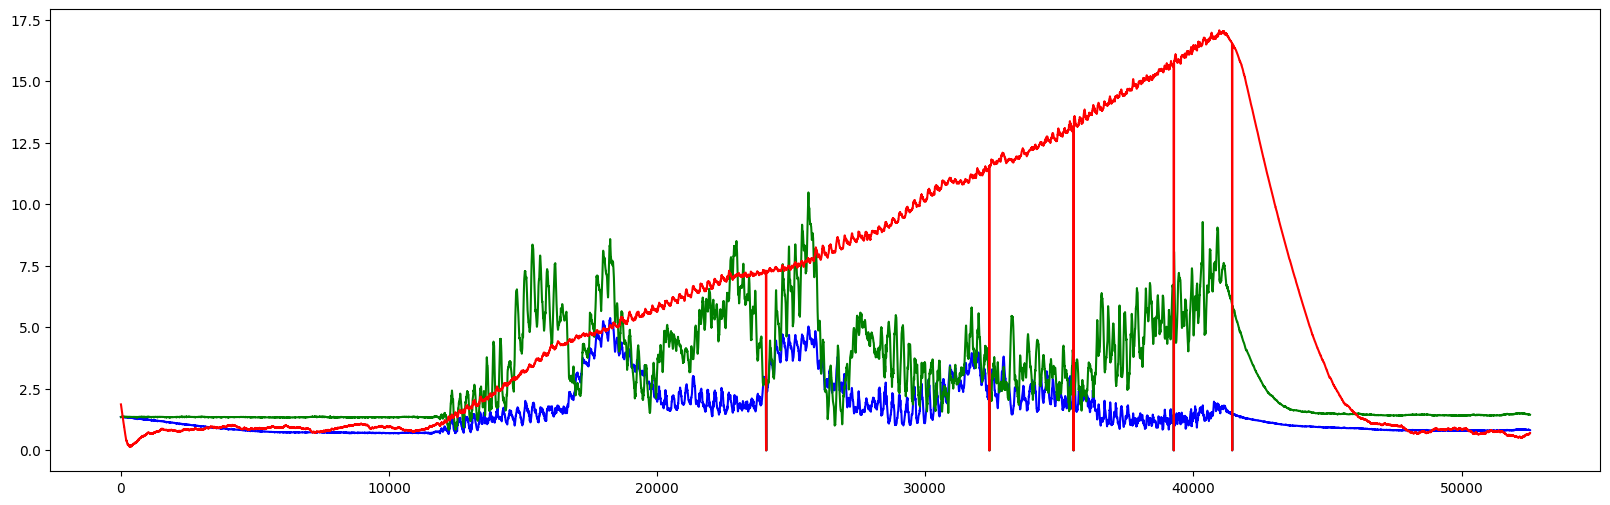
\includegraphics[width=0.9\linewidth]{figures/15_undisturbed_fast_translation_A.png}
    \caption{15\_undisturbed\_fast\_translation\_A}
    \label{fig:15_undisturbed_fast_translation_A}
\end{figure}

\begin{figure}[H]
    \centering
    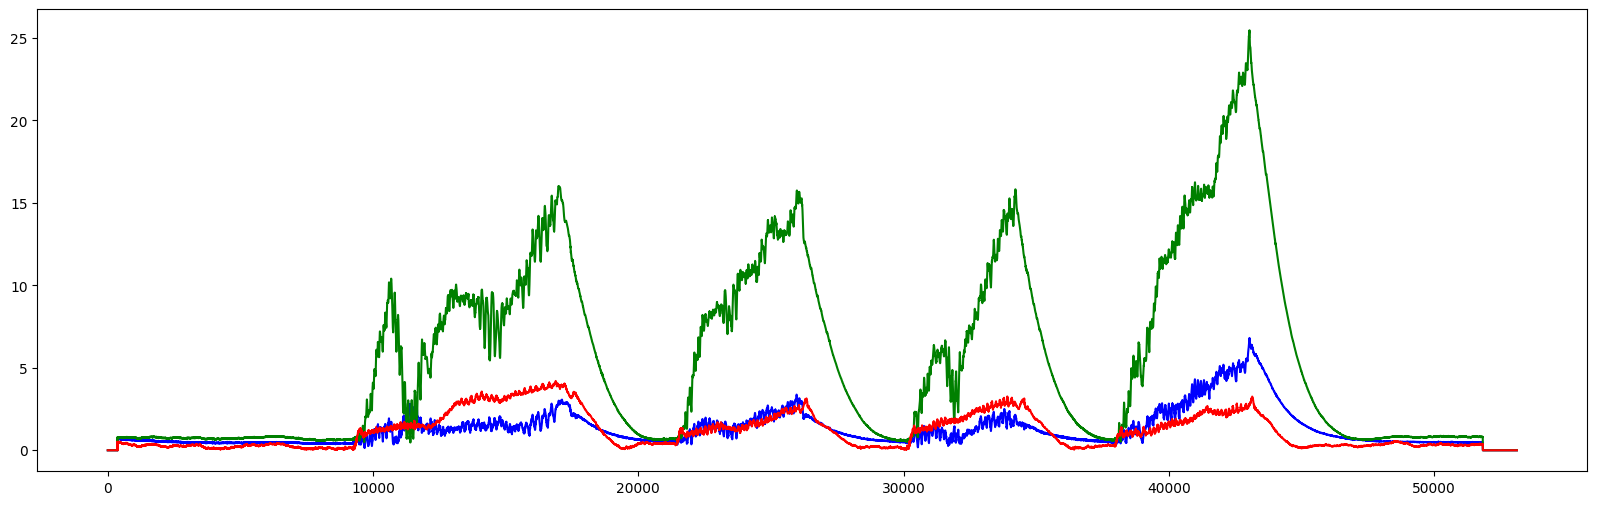
\includegraphics[width=0.9\linewidth]{figures/18_undisturbed_fast_translation_with_breaks_B.png}
    \caption{18\_undisturbed\_fast\_translation\_with\_breaks\_B}
    \label{fig:18_undisturbed_fast_translation_with_breaks_B}
\end{figure}

\begin{figure}[H]
    \centering
    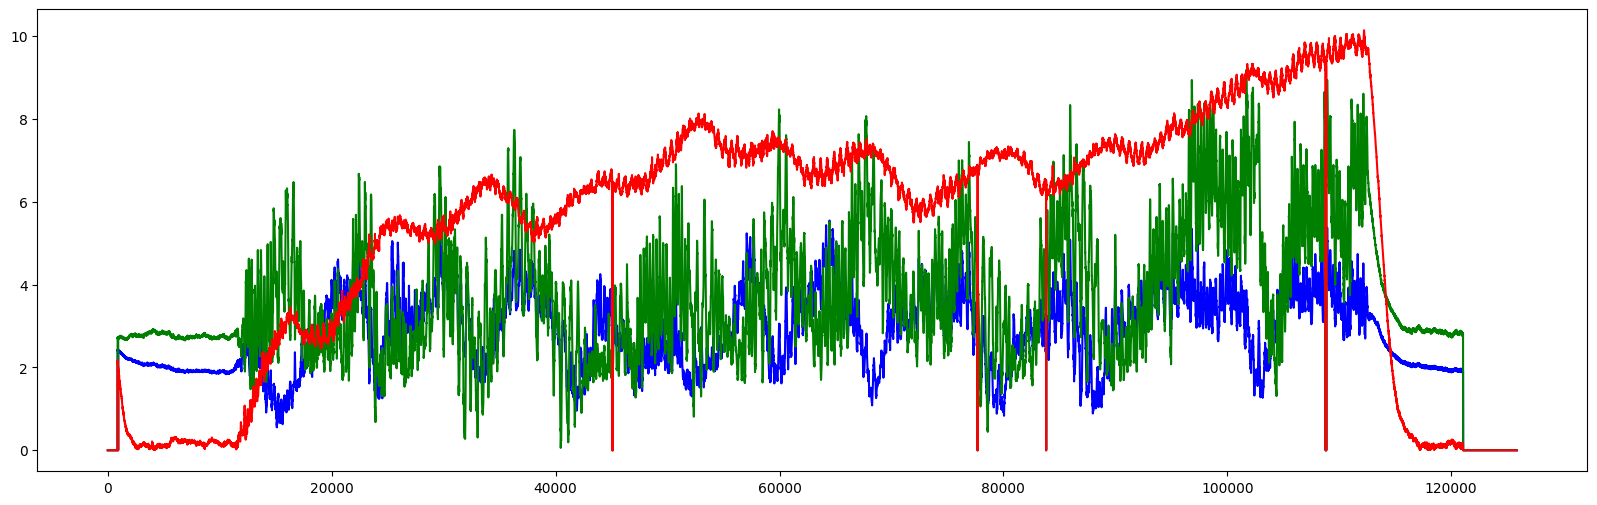
\includegraphics[width=0.9\linewidth]{figures/23_undisturbed_fast_combined_360s.png}
    \caption{23\_undisturbed\_fast\_combined\_360s}
    \label{fig:23_undisturbed_fast_combined_360s}
\end{figure}

\begin{figure}[H]
    \centering
    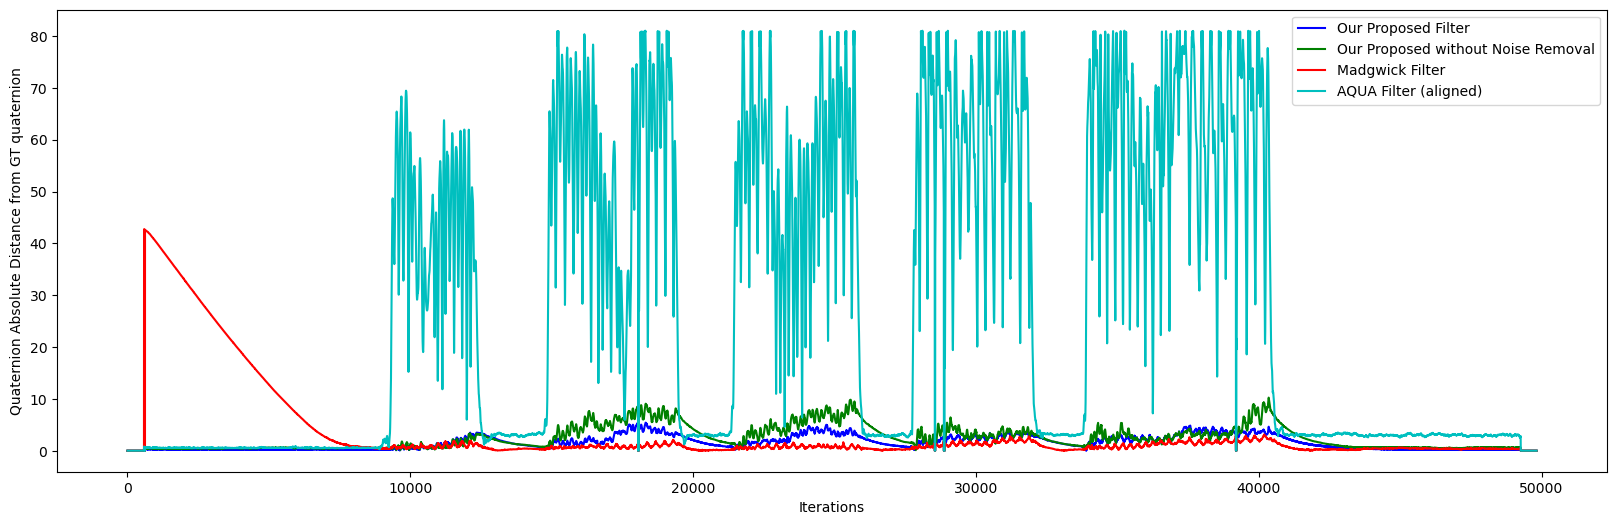
\includegraphics[width=0.9\linewidth]{figures/31_disturbed_stationary_magnet_D.png}
    \caption{31\_disturbed\_stationary\_magnet\_D}
    \label{fig:31_disturbed_stationary_magnet_D}
\end{figure}

\section{Performance of Our Filter against other filters on the Mechanical Platform} \label{section:mechanical_platform_result}
Here the results of running our proposed filter is tested along with the performaces of 
other standard existing filters - \emph{AQUA} \cite{aqua_ref}, \emph{EKF} \cite{ekf_ref} and the 
MadgWick Gradient Descent filter \cite{madgwick2011estimation}. 


 
\begin{table*}[ht]
\centering
\caption{Static error metrics (°) per axis when ML denoising is active.}
\label{tab:static_ml}
\begin{tabular}{l
  *{4}{ccc}
}
\toprule
Metric & \multicolumn{3}{c}{Proposed (ML)} & \multicolumn{3}{c}{Madgwick} & \multicolumn{3}{c}{EKF} & \multicolumn{3}{c}{Aqua} \\
 & X & Y & Z & X & Y & Z & X & Y & Z & X & Y & Z \\
\midrule
count & 6869.000 & 6869.000 & 6869.000 & ... & ... & ... & ... & ... & ... & ... & ... & ... \\
mean & 17.249 & 18.139 & 18.976 & ... & ... & ... & ... & ... & ... & ... & ... & ... \\
std & 13.995 & 14.498 & 19.820 & ... & ... & ... & ... & ... & ... & ... & ... & ... \\
min & 0.000457 & 0.000624 & 4.670 & ... & ... & ... & ... & ... & ... & ... & ... & ... \\
25\% & 0.044354 & 0.006244 & 4.670 & ... & ... & ... & ... & ... & ... & ... & ... & ... \\
50\% & 19.770 & 14.941 & 7.157 & ... & ... & ... & ... & ... & ... & ... & ... & ... \\
75\% & 30.153 & 32.723 & 30.253 & ... & ... & ... & ... & ... & ... & ... & ... & ... \\
max & 42.025 & 52.562 & 84.391 & ... & ... & ... & ... & ... & ... & ... & ... & ... \\
\bottomrule
\end{tabular}
\end{table*}






\begin{table*}[ht]
\centering
\caption{Static error metrics (°) per axis when ML denoising is not active.}
\label{tab:static_no_ml}
\begin{tabular}{l
  *{4}{ccc}
}
\toprule
Metric & \multicolumn{3}{c}{Proposed (-ML)} & \multicolumn{3}{c}{Madgwick} & \multicolumn{3}{c}{EKF} & \multicolumn{3}{c}{Aqua} \\
 & X & Y & Z & X & Y & Z & X & Y & Z & X & Y & Z \\
\midrule
count & 6869.000 & 6869.000 & 6869.000 & ... & ... & ... & ... & ... & ... & ... & ... & ... \\
mean & 17.249 & 18.139 & 18.976 & ... & ... & ... & ... & ... & ... & ... & ... & ... \\
std & 13.995 & 14.498 & 19.820 & ... & ... & ... & ... & ... & ... & ... & ... & ... \\
min & 0.000457 & 0.000624 & 4.670 & ... & ... & ... & ... & ... & ... & ... & ... & ... \\
25\% & 0.044354 & 0.006244 & 4.670 & ... & ... & ... & ... & ... & ... & ... & ... & ... \\
50\% & 19.770 & 14.941 & 7.157 & ... & ... & ... & ... & ... & ... & ... & ... & ... \\
75\% & 30.153 & 32.723 & 30.253 & ... & ... & ... & ... & ... & ... & ... & ... & ... \\
max & 42.025 & 52.562 & 84.391 & ... & ... & ... & ... & ... & ... & ... & ... & ... \\
\bottomrule
\end{tabular}
\end{table*}


\begin{table*}[ht]
\centering
\caption{Quasi Static error metrics (°) per axis when ML denoising is active.}
\label{tab:quasi_ml}
\begin{tabular}{l
  *{4}{ccc}
}
\toprule
Metric & \multicolumn{3}{c}{Proposed (ML)} & \multicolumn{3}{c}{Madgwick} & \multicolumn{3}{c}{EKF} & \multicolumn{3}{c}{Aqua} \\
 & X & Y & Z & X & Y & Z & X & Y & Z & X & Y & Z \\
\midrule
count & 6869.000 & 6869.000 & 6869.000 & ... & ... & ... & ... & ... & ... & ... & ... & ... \\
mean & 17.249 & 18.139 & 18.976 & ... & ... & ... & ... & ... & ... & ... & ... & ... \\
std & 13.995 & 14.498 & 19.820 & ... & ... & ... & ... & ... & ... & ... & ... & ... \\
min & 0.000457 & 0.000624 & 4.670 & ... & ... & ... & ... & ... & ... & ... & ... & ... \\
25\% & 0.044354 & 0.006244 & 4.670 & ... & ... & ... & ... & ... & ... & ... & ... & ... \\
50\% & 19.770 & 14.941 & 7.157 & ... & ... & ... & ... & ... & ... & ... & ... & ... \\
75\% & 30.153 & 32.723 & 30.253 & ... & ... & ... & ... & ... & ... & ... & ... & ... \\
max & 42.025 & 52.562 & 84.391 & ... & ... & ... & ... & ... & ... & ... & ... & ... \\
\bottomrule
\end{tabular}
\end{table*}


\begin{table*}[ht]
\centering
\caption{Quasi Static error metrics (°) per axis when ML denoising is not active.}
\label{tab:quasi_no_ml}
\begin{tabular}{l
  *{4}{ccc}
}
\toprule
Metric & \multicolumn{3}{c}{Proposed (-ML)} & \multicolumn{3}{c}{Madgwick} & \multicolumn{3}{c}{EKF} & \multicolumn{3}{c}{Aqua} \\
 & X & Y & Z & X & Y & Z & X & Y & Z & X & Y & Z \\
\midrule
count & 6869.000 & 6869.000 & 6869.000 & ... & ... & ... & ... & ... & ... & ... & ... & ... \\
mean & 17.249 & 18.139 & 18.976 & ... & ... & ... & ... & ... & ... & ... & ... & ... \\
std & 13.995 & 14.498 & 19.820 & ... & ... & ... & ... & ... & ... & ... & ... & ... \\
min & 0.000457 & 0.000624 & 4.670 & ... & ... & ... & ... & ... & ... & ... & ... & ... \\
25\% & 0.044354 & 0.006244 & 4.670 & ... & ... & ... & ... & ... & ... & ... & ... & ... \\
50\% & 19.770 & 14.941 & 7.157 & ... & ... & ... & ... & ... & ... & ... & ... & ... \\
75\% & 30.153 & 32.723 & 30.253 & ... & ... & ... & ... & ... & ... & ... & ... & ... \\
max & 42.025 & 52.562 & 84.391 & ... & ... & ... & ... & ... & ... & ... & ... & ... \\
\bottomrule
\end{tabular}
\end{table*}


\begin{table*}[ht]
\centering
\caption{Dynamic error metrics (°) per axis when ML denoising is active.}
\label{tab:dynamic_ml}
\begin{tabular}{l
  *{4}{ccc}
}
\toprule
Metric & \multicolumn{3}{c}{Proposed (ML)} & \multicolumn{3}{c}{Madgwick} & \multicolumn{3}{c}{EKF} & \multicolumn{3}{c}{Aqua} \\
 & X & Y & Z & X & Y & Z & X & Y & Z & X & Y & Z \\
\midrule
count & 6869.000 & 6869.000 & 6869.000 & ... & ... & ... & ... & ... & ... & ... & ... & ... \\
mean & 17.249 & 18.139 & 18.976 & ... & ... & ... & ... & ... & ... & ... & ... & ... \\
std & 13.995 & 14.498 & 19.820 & ... & ... & ... & ... & ... & ... & ... & ... & ... \\
min & 0.000457 & 0.000624 & 4.670 & ... & ... & ... & ... & ... & ... & ... & ... & ... \\
25\% & 0.044354 & 0.006244 & 4.670 & ... & ... & ... & ... & ... & ... & ... & ... & ... \\
50\% & 19.770 & 14.941 & 7.157 & ... & ... & ... & ... & ... & ... & ... & ... & ... \\
75\% & 30.153 & 32.723 & 30.253 & ... & ... & ... & ... & ... & ... & ... & ... & ... \\
max & 42.025 & 52.562 & 84.391 & ... & ... & ... & ... & ... & ... & ... & ... & ... \\
\bottomrule
\end{tabular}
\end{table*}


\begin{table*}[ht]
\centering
\caption{Dynamic error metrics (°) per axis when ML denoising is not active.}
\label{tab:dynamic_no_ml}
\begin{tabular}{l
  *{4}{ccc}
}
\toprule
Metric & \multicolumn{3}{c}{Proposed (-ML)} & \multicolumn{3}{c}{Madgwick} & \multicolumn{3}{c}{EKF} & \multicolumn{3}{c}{Aqua} \\
 & X & Y & Z & X & Y & Z & X & Y & Z & X & Y & Z \\
\midrule
count & 6869.000 & 6869.000 & 6869.000 & ... & ... & ... & ... & ... & ... & ... & ... & ... \\
mean & 17.249 & 18.139 & 18.976 & ... & ... & ... & ... & ... & ... & ... & ... & ... \\
std & 13.995 & 14.498 & 19.820 & ... & ... & ... & ... & ... & ... & ... & ... & ... \\
min & 0.000457 & 0.000624 & 4.670 & ... & ... & ... & ... & ... & ... & ... & ... & ... \\
25\% & 0.044354 & 0.006244 & 4.670 & ... & ... & ... & ... & ... & ... & ... & ... & ... \\
50\% & 19.770 & 14.941 & 7.157 & ... & ... & ... & ... & ... & ... & ... & ... & ... \\
75\% & 30.153 & 32.723 & 30.253 & ... & ... & ... & ... & ... & ... & ... & ... & ... \\
max & 42.025 & 52.562 & 84.391 & ... & ... & ... & ... & ... & ... & ... & ... & ... \\
\bottomrule
\end{tabular}
\end{table*}



\begin{table}[ht]
  \centering
  \caption{Resource consumption per filter on RPI: average CPU (\%) and memory (MB).}
  \label{tab:resource_consumption}
  \begin{tabular}{lcc}
    \toprule
    Filter & CPU Usage (\%) & Memory Usage (MB) \\
    \midrule
    Proposed (ML)     & \([\,\cdot\,]\) & \([\,\cdot\,]\) \\
    Proposed (-ML)    & \([\,\cdot\,]\) & \([\,\cdot\,]\) \\
    Madgwick           & \([\,\cdot\,]\) & \([\,\cdot\,]\) \\
    EKF                & \([\,\cdot\,]\) & \([\,\cdot\,]\) \\
    Aqua               & \([\,\cdot\,]\) & \([\,\cdot\,]\) \\
    \bottomrule
  \end{tabular}
\end{table}

\begin{table}[ht]
  \centering
  \caption{Long-term drift over \(T\) hours (°/h).}
  \label{tab:long_term_drift}
  \begin{tabular}{lcc}
    \toprule
    Filter & Drift (°/hr) \\
    \midrule
    Proposed (ML)     & \([\,\cdot\,]\) \\
    Proposed (-ML)    & \([\,\cdot\,]\) \\
    Madgwick           & \([\,\cdot\,]\) \\
    EKF                & \([\,\cdot\,]\) \\
    Aqua               & \([\,\cdot\,]\) \\
    \bottomrule
  \end{tabular}
\end{table}




\chapter{Interpretation Of Results} \label{chapter:discussion}

In this chapter, the results achieved in \autoref{chapter:results} will be interpreted in detail. The results we have acheived so far is promising, and it is able to outperform standard Madgwick filter implementation in fast motion scenarios which was one of our goals initially.

\section{Results Without Denoising}
In \autoref{result:meanerrortoggle} and \autoref{result:varerrortoggle} we can observe spikes in the orange line graph
which represent the Madgwick Filter. Our proposed filter (in Green) is able to avoid high spikes in files \texttt{15\_undisturbed\_fast\_translation\_A},\texttt{23\_undisturbed\_fast\_combined\_360s} and in \texttt{27\_disturbed\_phone\_vibration\_B} 
in comparisions of mean error in \autoref{result:meanerrortoggle}. This indicates that in fast motion scenarios the toggling of $\alpha$ 
has a positive effect on the error in our proposed filter avoiding higher mean error. In case of variance comparison
in \autoref{result:varerrortoggle} we see that our proposed(Green line) has the least variance among all three.

\subsection{Intuitive Reasoning Backed by Emperical Evidence}
Here we suggest why $\alpha$-toggling might result in a better performance.
\begin{itemize}
    \item Toggling the $\alpha$ is done in scenarios when there is movement. When the model predicts there is some movement 
    instead of varying the alpha, the alpha is toggled according to defined duty cycle and frequency, this gives just enough information for the gyroscope error to correct itself.
    \item When there is no movement(predicted by the model), then the $\alpha$ is set to its predefined value. Here the assumption is that the system is much less noisy when there is less movement, and thus can employ more trust to the accelerometer and magnetometer by keeping the alpha to a constant value.
\end{itemize}


\section{Results With Denoising}

The results shown after denoising is much more promising than the results without denoising. In 
\autoref{tab:error_statistics_cvset_mean} and \autoref{tab:error_statistics_cvset_variance} we can observe 
that our proposed filter performs better than atleast one of the filters in all five trials of the \texttt{cv\_set}.
In case of variance of errors in \autoref{tab:error_statistics_cvset_variance}, our filter consistently is able to maintain error variance around 1.0 where the other compared 
filters often exceed and reach a variance 10x or 20x of our proposed filter.

From the tables, it is observed that in \autoref{tab:error_statistics_cvset_mean}, the best performance of
our filter is visible in entries 2 and 4 which correspond to the files \texttt{15\_undisturbed\_fast\_translation\_A} and \texttt{23\_undisturbed\_fast\_combined\_360s} respectively.
Thus our filter is able to outperform the standard Madgwick filter implementation in fast motion scenarios.

If we observe the error graphed vs iterations for \texttt{15\_undisturbed\_fast\_translation\_A} in \autoref{fig:15_undisturbed_fast_translation_A} in \autoref{subsec:individualFiles}, we observe that the
Madgwick Filter's error steadily rises where our proposed complementary filter stays close to zero. For the file \autoref{fig:18_undisturbed_fast_translation_with_breaks_B},
we observe that Madgwick filter performs marginally better.

\subsection{Intuitive Reasoning Based on Emperical Evidence}

\begin{itemize}
    \item As noise is subtracted from the accelerometer and magnetometer readings, the extraneous linear acceleration is subtracted, as a 
    result the orientation estimation is far superior in case of fast motions.
    \item It is observed from \autoref{fig:18_undisturbed_fast_translation_with_breaks_B} that the MadgWick filter stabilizes and converges to a good orientation when there is no motion, thus in the file \\ \texttt{18\_undisturbed\_fast\_translation\_with\_breaks\_B} the Madgwick filter performs better than our filter as it
    has breaks to recover from its error. In case of \autoref{fig:15_undisturbed_fast_translation_A} for the file 
    \texttt{15\_undisturbed\_fast\_translation\_A} the Madgwick filter is not able to stabilize itself,as there are no breaks and hence our filter performs better.
\end{itemize}

\chapter{Shortcomings in our Approach}
Our approach is data driven, thus it would require us more time and memory complexity to perform inference from our models, which will nullify the mathematical simplicity of the complementary filter.

\begin{itemize}
    \item \textbf{Size of the model:} The inference time of a tree based model is $O(log(n))$ where $n$ is the number of nodes in the tree. The inference time is thus bound by the depth of the tree which was limited to 15. Thus for 6 variables and 15 estimators we would need $15*6*6$ decisions. This is not a large number , but the cause of concern would be the memory complexity as the trees of the XGBoost models are observed to be very wide.
    \item \textbf{Cost of Matrix Exponentiation:} Matrix exponentiation is used to rotate the vectors.
    \item  \textbf{Training Time:} Training with RANSAC requires considerable amount of time.
    \item \textbf{Generalizability:} The models perform well in test set compared to the cv set.
\end{itemize}




\chapter{Future Works} \label{chapter:futureWorks}
Our current approach offers significant improvements in orientation estimation by integrating data-driven approaches with complementary filtering techniques. However, as with any research, there remain numerous opportunities to expand, improve, and apply these methods in broader contexts. The following subsections discuss possible future directions in more detail.

\section{Real-World Deployment and Extended Testing}
While this thesis primarily evaluates the proposed algorithms on the BROAD dataset and a controlled mechanical turntable setup, real-world deployments present additional challenges. Future work should focus on implementing the algorithm on portable devices such as smartphones, 
drones, or wearable sensors, and then testing it across diverse environments including indoor, outdoor, urban, and industrial settings. Real-world data will inevitably contain more complex disturbances, unexpected motion patterns, and magnetic interference, providing a more stringent test of the algorithm’s robustness and adaptability. Continuous monitoring over extended periods could also reveal long-term drift behaviors and system stability under typical usage conditions.

Building and deploying custom hardware based on embedded microcontrollers or small form-factor single board computers (e.g., ESP32, Raspberry Pi) would lay the groundwork for practical applications. This would help uncover challenges related to sensor calibration, sensor placement, power constraints, and wireless data transmission that are less obvious in simulations or lab setups.


\section{Further Optimization of Machine Learning Models for Embedded Systems}
One of the key challenges identified is the resource demand of the current XGBoost models, especially on low-memory and low-power embedded platforms. Future research should investigate techniques for model compression and acceleration, such as pruning, quantization, and knowledge distillation. These methods reduce model size and computation without drastically sacrificing accuracy.

Alternatively, experimenting with other lightweight and interpretable models like decision trees, linear models with feature engineering, or hybrid heuristic approaches could offer better trade-offs between inference speed, memory pressure, and prediction reliability. Developing customized inference engines or hardware accelerators specialized for tree-based models might also help enable real-time execution on microcontrollers with limited flash and RAM.

\section{Online and Adaptive Learning Approaches}
Currently, the models are trained offline using pre-collected datasets and applied without updates during operation. Future research could explore online learning or incremental training where the model continues to adapt in real time based on new sensor data. This could allow the system to cope better with sensor aging, environmental changes, or new motion types without manual retraining.

Adaptive algorithms could leverage unsupervised or semi-supervised learning to detect drifts in sensor behavior or novel disturbance patterns and dynamically update the fusion gain or noise compensation parameters. Such self-tuning models would enhance long-term reliability and reduce maintenance requirements.

\section{Integration of Additional Sensor Modalities}
While this thesis focuses on fusing accelerometer, gyroscope, and magnetometer data (MARG), adding complementary sensor modalities could further improve orientation accuracy and robustness. For instance, integrating GPS or ultra-wideband (UWB) sensors could offer absolute position or heading references to correct drift.

Vision-based sensors like cameras or depth sensors could provide rich environmental context and aid in occlusion detection or loop closure in navigation scenarios. Incorporating barometric pressure sensors could help improve altitude estimation which indirectly influences orientation filters. Future work can explore multi-sensor fusion algorithms that intelligently weight sensor inputs based on context and confidence levels.

\section{Enhanced Noise and Disturbance Modeling}
Though this work reduces noise via a data-driven regression model, further improvements could be achieved by developing more advanced noise models. Future research might consider modeling temporal noise correlations using recurrent neural networks or probabilistic graphical models to capture sequential dependencies.

Domain-specific noise types, such as vibration noise on drones or magnetic disturbances in industrial environments, could be separately characterized and mitigated. Investigating robust statistics or outlier detection mechanisms integrated with sensor fusion may help reject spurious sensor inputs and further enhance filtering performance.

\section{Exploration of Alternative Data-Driven Fusion Architectures}
The approach in this thesis uses a hybrid of classical complementary filtering and tree-based machine learning models. Future work could investigate end-to-end deep learning architectures that directly regress orientation quaternions or rotation matrices from raw sensor sequences. Approaches using convolutional neural networks (CNNs), recurrent networks (RNNs), transformers, or attention mechanisms have shown promising results in recent literature.

However, these models often require large labeled datasets and heavy computational resources, so approaches combining classical filters with learned corrections or uncertainty-aware models might strike the best balance. Research can explore explainability and interpretability of such models to maintain trust in safety-critical applications.

\section{Comprehensive Performance Benchmarking and Standardization}
To better understand the trade-offs and advantages of the proposed algorithms, large-scale benchmarking on standardized datasets with various metrics (accuracy, latency, resource usage, robustness) needs to be conducted. Extending experiments to multiple IMU platforms and sensor qualities would highlight generalizability and scalability.

\\
By pursuing these research directions, future work can build upon the foundation laid in this thesis to develop even more accurate, efficient, and adaptive orientation estimation systems suitable for real-world applications across robotics, augmented reality, autonomous vehicles, and wearable technologies.











%-------------------------- BACK MATTER --------------------------%

% Print the references used throughout the document, mandatory
\printbib

% You may attach chapter as appendices inside the following environment
\begin{appendices}

\chapter{Quaternion} 

\section{Quaternion Fundamentals}

\subsection{Basic Operations with Quaternions}

A quaternion $q$ is a four-dimensional number composed of a scalar part and a three-dimensional vector part:
\[
q = w + xi + yj + zk
\]
where $w, x, y, z \in \mathbb{R}$, and $i, j, k$ are imaginary units satisfying:
\[
i^2 = j^2 = k^2 = ijk = -1
\]

The basic operations on quaternions are:

\begin{itemize}
    \item \textbf{Addition:} Given two quaternions $q_1 = (w_1, \mathbf{v}_1)$ and $q_2 = (w_2, \mathbf{v}_2)$, their sum is
    \[
    q_1 + q_2 = (w_1 + w_2, \mathbf{v}_1 + \mathbf{v}_2)
    \]
    
    \item \textbf{Multiplication:} The product $q = q_1 \otimes q_2$ is defined as
    \[
    q = (w_1w_2 - \mathbf{v}_1 \cdot \mathbf{v}_2,\; w_1\mathbf{v}_2 + w_2\mathbf{v}_1 + \mathbf{v}_1 \times \mathbf{v}_2)
    \]
    where $\cdot$ denotes the dot product and $\times$ denotes the cross product.
    
    \item \textbf{Conjugate:} The conjugate of $q = (w, \mathbf{v})$ is
    \[
    q^* = (w, -\mathbf{v})
    \]
    
    \item \textbf{Norm:} The norm of $q$ is given by
    \[
    \|q\| = \sqrt{w^2 + x^2 + y^2 + z^2}
    \]
    
    \item \textbf{Inverse:} For a nonzero quaternion,
    \[
    q^{-1} = \frac{q^*}{\|q\|^2}
    \]
\end{itemize}

\subsection{Rotating a Vector Using a Quaternion} \label{subsec:rotatevector}

To rotate a 3D vector $\mathbf{v} \in \mathbb{R}^3$ using a unit quaternion $q$, the following procedure is used:

\begin{enumerate}
    \item Represent $\mathbf{v}$ as a pure quaternion:
    \[
    v_q = (0, \mathbf{v})
    \]
    
    \item Apply the rotation:
    \[
    v_{\text{rotated}} = q \otimes v_q \otimes q^*
    \]
    where $q^*$ is the conjugate of $q$, and $\otimes$ denotes quaternion multiplication.
    
    \item Extract the vector part of $v_{\text{rotated}}$ to obtain the rotated vector.
\end{enumerate}

The quaternion rotation formula ensures a smooth and gimbal-lock-free rotation, which is particularly advantageous in 3D applications such as orientation tracking and robotics.


\section{Absolute Distance} \label{appendix:quaternion-distance}
In this section, we describe the computation of the \textit{Quaternion Absolute Distance} (QAD), a common metric used to evaluate differences between two orientation quaternions.

Given two unit quaternions:
\begin{itemize}
    \item $\mathbf{q}_1 = [w_1, x_1, y_1, z_1]$
    \item $\mathbf{q}_2 = [w_2, x_2, y_2, z_2]$
\end{itemize}

The absolute distance $Quat_{abs\_dist}$ between them is defined as:

\begin{equation}
    Quat_{abs\_dist}(\mathbf{q}_1, \mathbf{q}_2) = 1 - \left| \langle \mathbf{q}_1, \mathbf{q}_2 \rangle \right| = 1 - \left| w_1 w_2 + x_1 x_2 + y_1 y_2 + z_1 z_2 \right|
\end{equation}

This distance is derived from the dot product between the two quaternions and captures the angular difference in orientation. Since quaternions $\mathbf{q}$ and $-\mathbf{q}$ represent the same rotation, taking the absolute value of the dot product ensures the distance is invariant to this ambiguity.

\subsection{Properties}
\begin{itemize}
    \item $Quat_{abs\_dist}(\mathbf{q}_1, \mathbf{q}_2) = 0$ if $\mathbf{q}_1 = \mathbf{q}_2$ or $\mathbf{q}_1 = -\mathbf{q}_2$
    \item $Quat_{abs\_dist} \in [0, 1]$ for normalized quaternions
    \item The closer the value is to $0$, the more similar the orientations
\end{itemize}

\subsection{Use Cases}
Quaternion Absolute Distance is frequently used in:
\begin{itemize}
    \item Orientation estimation
    \item Motion capture and sensor fusion
    \item Evaluating the accuracy of inertial tracking algorithms
\end{itemize}
\end{appendices}

\end{document}


